%%%%%%%%%%%%%%%%%%%%%%%%%%%%%%  IEEEsample.tex  %%%%%%%%%%%%%%%%%%%%%%%%%%%%%%%
%%%%%%%%%%                                                        %%%%%%%%%%%%%
%%%%%%%%%%    More information: see the header of IEEEtran.sty    %%%%%%%%%%%%%
%%%%%%%%%%                                                        %%%%%%%%%%%%%
%%%%%%%%%%%%%%%%%%%%%%%%%%%%%%%%%%%%%%%%%%%%%%%%%%%%%%%%%%%%%%%%%%%%%%%%%%%%%%%
%
%\documentstyle[twocolumn]{IEEEtran}

%\documentclass[a4paper,12pt]{article}

% The amsmath and epsfig packages greatly simplify the process of adding
% equations and figures to the document, and thus their use is highly
% recommended.
% ------------

\documentclass[11pt, runningheads,a4paper]{llncs}

\usepackage{tikz}
\usepackage{amsmath}
\usepackage{epsfig}
\usepackage{acronym}
\usepackage{array}
\usepackage{listings}
\usepackage[latin1]{inputenc}
\usepackage{amsmath}
\usepackage{amsfonts}
\usepackage{amssymb}
\usepackage{graphicx} 
\usepackage[latin1]{inputenc}
\usepackage{amsmath}
\usepackage{amsfonts}
\usepackage{amssymb}  
\usepackage{fancyhdr}
\usepackage{listings}
\usepackage{url}
\usepackage{float}
\usepackage[top=2cm, bottom=2cm, left=2cm, right=2cm]{geometry}


\usepackage{acronym}
\usepackage{caption}
\usepackage{subcaption}
\usepackage{subfig}
\usepackage{graphicx}
\usepackage{setspace}
\usepackage{underlin}
\usepackage{algpseudocode}
\usepackage{algorithm}
\usepackage{amssymb}
\usepackage{booktabs}
\usepackage{makeidx} 
\usepackage{microtype} 


\newcommand{\HRule}{\rule{\linewidth}{0.5mm}}

\acrodef{fpga}[FPGA]{Field programmable gate array}
\acrodef{cpld}[CPLD]{complex programmable logic device}
\acrodef{asic}[ASIC]{application specific integrated circuits}
\acrodef{isa}[ISA]{instruction set architecture}
\acrodef{gpu}[GPU]{graphic processing unit}
\acrodef{fpu}[FPU]{floating processing unit}
\acrodef{hdl}[HDL]{hardware description language}
\acrodef{api}[API]{application programming interface}
\acrodef{ip}[IP]{intellectual property}
\acrodef{lut}[LUT]{lookup tables}
\acrodef{bram}[BRAM]{block RAM}
\acrodef{dsu}[DSU]{debug support unit}
\acrodef{alu}[ALU]{arithmetic logical unit}
\acrodef{cam}[CAM]{custom address memory}
\acrodef{hll}[HLL]{higher level languages}
\acrodef{cpu}[CPU]{central processing unit}
\acrodef{par}[PAR]{place and route}
\acrodef{ai}[AI]{artificial intelligence}
\acrodef{ipc}[IPC]{instruction per cycle}
\acrodef{fd}[FD]{finite difference}
\acrodef{ea}[EA]{evolutionary algorithms}
\acrodef{ann}[ANN]{artificial neural network}
\acrodef{svm}[SVM]{support vector machines}
\acrodef{veb}[VEB]{virtual embedded block}
\acrodef{mmu}[MMU]{Memory Management Unit}
\acrodef{cpld}[CPLD]{complex programmable logic device}
\acrodef{asic}[ASIC]{application specific integrated circuits}
\acrodef{isa}[ISA]{instruction set architecture}
\acrodef{gpu}[GPU]{graphic processing unit}
\acrodef{fpu}[FPU]{floating processing unit}
\acrodef{hdl}[HDL]{hardware description language}
\acrodef{api}[API]{application programming interface}
\acrodef{ip}[IP]{intellectual property}
\acrodef{lut}[LUT]{lookup tables}
\acrodef{bram}[BRAM]{block RAM}
\acrodef{dsu}[DSU]{debug support unit}
\acrodef{alu}[ALU]{arithmetic logical unit}
\acrodef{cam}[CAM]{custom address memory}
\acrodef{hll}[HLL]{higher level languages}
\acrodef{cpu}[CPU]{central processing unit}
\acrodef{par}[PAR]{place and route}
\acrodef{ai}[AI]{artificial intelligence}
\acrodef{ipc}[IPC]{instruction per cycle}
\acrodef{fd}[FD]{finite difference}
\acrodef{ea}[EA]{evolutionary algorithms}
\acrodef{ann}[ANN]{artificial neural network}
\acrodef{svm}[SVM]{support vector machines}
\acrodef{veb}[VEB]{virtual embedded block}
\acrodef{mmu}[MMU]{Memory Management Unit}
\acrodef{rmt}[RMT]{remapping table}
\acrodef{lnreg}[LNreg]{Line Number Register}
\acrodef{secrand}[SecRAND]{Security-Aware Random Replacement Algorithm}
\acrodef{aes}[AES]{Advanced Encryption System}
\acrodef{asi}[ASI]{Address space identifier}
\acrodef{fsm}[FSM]{Finite State Machines}
\acrodef{pca}[PCA]{Principal Component Analysis}
\acrodef{asip}[ASIP]{Application Specific Instruction Processor}
\acrodef{gp}[GP]{Gaussian Process}
\acrodef{gbsa}[GbSA]{Galaxy-based Search Algorithm}
\acrodef{aco}[ACO]{Ant Colony Optimization}
\acrodef{pso}[PSO]{Particle Swarm Optimization}
\acrodef{sa}[SA]{Simulated Annealing}
\acrodef{ga}[GA]{Genetic Algorithm}
\acrodef{iwdp}[IWDP]{Intelligent Water Drops}
\acrodef{hpc}[HPC]{High Performance Computing}
\acrodef{ib}[IB]{Investment Banking}
\acrodef{par}[PAR]{Place and Route}
\acrodef{agppso}[A-GP-PSO]{Adaptive Gaussian Process Particle Swarm Optimizer}
\acrodef{vpso}[VPSO]{Adaptive Velocity Particle Swarm Algorithm}
\acrodef{aes}[AES]{Advanced Encryption System}
\acrodef{cad}[CAD]{Computer Aided Design}
\acrodef{svm}[SVM]{Support Vector Machine}
\acrodef{alo}[MLO]{Machine Learning Optimizer}
\acrodef{moalo}[MOMLO]{Multi-Objective Machine Learning Optimizer}
\acrodef{mopso}[MOMLO]{Multi-Objective Particle Swarm Optimizer}
\acrodef{rvm}[RVM]{Relevance Vector Machine}
\acrodef{rbf}[RBF]{Radial Basis Function}
\newcommand{\ra}[1]{\renewcommand{\arraystretch}{#1}}

\newcommand{\keywords}[1]{\par\addvspace\baselineskip
\noindent\keywordname\enspace\ignorespaces#1}


\pagestyle{headings}
\linespread{1}
\begin{document}
\thispagestyle{empty}
\begin{center}

\includegraphics[width=0.15\textwidth]{imperial-college-london-logo.png}~\\[1cm]
\textsc{\LARGE Imperial College London}\\[1.5cm]

\textsc{\Large Independent Study Option}\\[0.5cm]

% Title
\HRule \\[0.4cm]
{ \huge \bfseries Machine Learning Optimizer for FPGA architecture exploration}\\[0.4cm]

\HRule \\[1.5cm]

% Author and supervisor
\begin{minipage}{0.4\textwidth}
\begin{flushleft} \large
\emph{Author:}\\
Tianchi \textsc{Liu}
\end{flushleft}
\end{minipage}
\begin{minipage}{0.4\textwidth}
\begin{flushright} \large
\emph{Supervisor:} \\
Prof.~Wayne \textsc{Luk}
\end{flushright}
\end{minipage}

\vfill

% Bottom of the page
{\large \today}

\end{center}



%\mainmatter  % start of an individual contribution
\setcounter{page}{1}
\title{Machine Learning Optimizer for FPGA architecture exploration}

% a short form should be given in case it is too long for the running head

% the name(s) of the author(s) follow(s) next
%
% NB: Chinese authors should write their first names(s) in front of
% their surnames. This ensures that the names appear correctly in
% the running heads and the author index.
%
\author{Tianchi Liu}
%
% (feature abused for this document to repeat the title also on left hand pages)

% the affiliations are given next; don't give your e-mail address
% unless you accept that it will be published
\institute{Department of Computing, Imperial College London}

\maketitle
\begin{abstract}


 We present a multi-objective machine learning optimization strategy developed based on the previous work on the \ac{alo}, which presents a novel technique that uses meta-heuristics and machine learning to automate the optimization of design parameters for reconfigurable designs. The main inspiration for this paper is to extend the application to be able to find trade-offs between different \ac{fpga} performance measures and get well formed Pareto Optimal Set for the parameter space of FPGA architecture.  In order to achieve this, we present several versions of \ac{moalo} best on Pareto optimal solution in order to find a best one which can present a best approximation of the Pareto Front. Further work is done on the regression test on the MLO to compare the current result to the golden result in order to evaluate how good the new design is. We evaluate our approach using four case studies and compare the results from different version of \ac{mopso}. It is noticeable that this is a completely novel way of exploring the FPGA architecture within multi-objective scope and the result gain from artificial continuous functions has proved it will be successful in FPGA design.


\keywords{Optimization, Multi-Objective PSO, GP, SVM, FPGA}

\end{abstract}

 As a result the parameter space exploration of FPGA can take a tremendous amount of time, we have shown it to be useful to construct surrogate models of fitness functions representing design quality of reconfigurable hardware designs \cite{arc2012MLO}, \cite{fpt2012MLO}. As these models are orders of magnitude faster to evaluate than the actual benchmarks and bitstreams, they can substantially accelerate optimization thus allowing for an automated approach. This is the motivation behind our development of the MLO tool which we apply to the problem of reconfigurable designs parameter optimization. Recently however; issues like power efficiency or size have become more prominent, and consequently the design which give trade-off among different \ac{fpga} quality measures is extremely important at this perspective. In this paper we expanding the previous \ac{fpga} architecture exploration problem into the multi-objective optimization domain. We present a new multi-objective flavor of MLO and evaluate it using a number of examples. The contributions of this paper are:

\vspace{-0.5em}

\begin{list}{$\bullet$}{\itemsep 0.5ex}

\item A mathematical characterization of multi-objective optimization in reconfigurable applications. We extend the previous description \cite{arc2012MLO} (Section III).

\item A implementation of new multi-objective version of MLO. We show how multiple Bayesian regressors and multi-objective meta heuristics can be interlinked (Section IV).

\item An evaluation of the extended MOMLO approach using four multi-objective fitness functions(Section V): (a) Two single-objective functions in minimization problem, and (b) Two single-objective functions in maximization problem, and (c) One bi-objective function  and (d) One three-objective function.
\end{list}




\section{Background}
\subsection{FPGA}
 Field-Programmable Gate Arrays (FPGAs) are pre-fabricated devices that can be used to implement logic without going through an expensive fabrication process. The reconfigurability and customization of FPGA designs potentially increases performance and efficiency without increasing the frequency and consume much low power than the traditional processor \cite{arc2012MLO}. However, due to the substantial effort for the FPGA designers to analyze the application and build the corresponding models and benchmarks, it is unlikely for the designer to finish all of the procedures to optimize design within a reasonable time and performance. 
After taking a scrutiny of the design process,  some designers use a exhaustive search method to explore the parameters such as numerical precision, degree of pipelining or number of cores. Nevertheless, when it comes to realistic problem it is not always applicable because benchmark evaluations and code execution take hours of compute time. Surrogate models approximating fitness functions by substituting lengthy evaluations with estimations based on closeness in a design space have been investigated in reconfigurable computing \cite{Pilato2008}. Together with machine learning techniques, surrogate modelling then can be used to reduce the original efforts of designers.

%\vspace{-1em}

\subsection{Gaussian Process Regression}

\ac{gp} is a machine learning technology based on strict theoretical fundamentals and Bayesian theory \cite{Seeger04gaussianprocesses,Rasmussen06gaussianprocesses}. \ac{gp} does not require a predefined structure, can approximate arbitrary function landscapes including discontinuities, and includes a theoretical framework for obtaining the optimum hyper-parameters \cite{5194095}. An advantage of \ac{gp} is that it provides a predictive distribution, not a point estimate.

A Gaussian process is a collection of random variables, any finite set of which have a joint Gaussian distribution \cite{Seeger04gaussianprocesses}. A Gaussian process is completely specified by its mean function $m(\mathbf{x})$ and the covariance (kernel) function $k(\mathbf{x},\mathbf{x'})$:

%\vspace{-1em}


\begin{align} 
\hat{f}(\mathbf{x}) \sim \mathcal{G}\mathcal{P}(m(\mathbf{x}),k(\mathbf{x},\mathbf{x'}))
\end{align}

%\vspace{-0.5em}

The $k(\mathbf{x},\mathbf{x'})$ expresses the covariance between pairs of random variables, and in regression analysis it expresses the relation between input-output pairs. This is based on a training set $\mathcal{D}$ of $n$ observations, $\mathcal{D}={(\mathbf{x}_i,y_{i}) | i = 1, ... n} $, where $\mathbf{x}$ denotes an input vector, $y$ denotes a scalar output. The column vector inputs for all $n$ cases are aggregated in the $D \times n$ design matrix $X$, and the outputs are collected in the vector $\mathbf{y}$. The goal of Bayesian forecasting is to compute the distribution $p(\hat{f}|\mathbf{x_*},\mathbf{y},X)$ of the function $\hat{f}$ at unseen input $\mathbf{x_{*}}$ given a set of training points $\mathcal{D}$. Using Bayes rule, the predictive posterior for the Gaussian process $\hat{f}$ and the predicted scalar outputs $\hat{f}(\mathbf{x_*})=y_*$ can be obtained.

% By conditioning on the observed targets in the training set, the predictive distribution is Gaussian.

%\vspace{-1em}


\subsection{Support Vector Machines Classification}

\ac{svm} is a maximum margin classifier, which constructs a hyperplane used for classification (or regression) \cite{Bishop:2006:PRM:1162264}. \acp{svm} use kernel functions $k(\mathbf{x},\mathbf{x'})$ to transform the original feature space to a different space where a linear model is used for classification. \acp{svm} are a class of decision machines and so do not provide posterior probabilities. There is a training set $\mathcal{D}$ of $n$ observations, $\mathcal{D}={(\mathbf{x}_i,t_{i}) | i = 1, ... n} $, where $\mathbf{x}$ denotes an input vector, $t$ denotes a target value. The column vector inputs for all $n$ cases are aggregated in the $D \times n$ design matrix $X$, and the targets in the vector $\mathbf{t}$. The goal is to classify an unseen input $\mathbf{x_{*}}$ based on $X$ and $\mathbf{t}$ by computing a decision boundary. 

%\begin{align} 
%f(x) = w^{T} \phi(x) + \beta
%\end{align}

%\vspace{-1em}


\subsection{Particle Swarm Algorithm (PSO)}
%with inertia governing its movement
Particle Swarm Optimization (PSO) is a heuristic search technique (which is considered as an evolutionary algorithm by its authors \cite{pso1998}) that simulates the movements of a flock of birds which aim to find food. The relative simplicity of PSO and the fact that is a population-based technique have made it a natural candidate to be extended for multi-objective optimization.
In the following we provide some definitions of several technical terms commonly used:
\begin{list}{$\bullet$}{\itemsep 0.5ex}

\item $Swarm$:  Population of the algorithm.

\item $Particle$:  Member (individual) of the swarm. Each particle represents a potential solution to the problem being solved. The position of a particle is determined by the solution it currently represents.

\item $pbest$  (personal best ):  Personal best position of a given particle, so far. That is, the position of the particle that has provided the greatest success (measured in terms of a scalar value analogous to the fitness adopted in evolutionary algorithms).

\item $lbest$  (local best ):  Position of the best particle member of the neighborhood of a given particle.

\item $gbest$  (global best ):  Position of the best particle of the entire swarm.
\item $Leader$:  Particle that is used to guide another particle towards better regions of the search space.

\item $Velocity$ (vector):  This vector drives the optimisation process, that is, it determines the direction in which a particle needs to "fly" (move), in order to improve its current position.
\item $Inertia weight$:  Denoted by W , the inertia weight is employed to control the impact of the previous history of velocities on the current velocity
\item $Learning\ factor$: Represents the attraction that a particle has toward either its own success or that of its neighbors. Two are the learning factors used: $C1$ and $C2$. $C1$ is the cognitive learning factor and represents the attraction that a particle has toward its own success. $C2$ is the social learning factor and represents the attraction that a particle has toward the success of its neighbors. Both, $C1$ and $C2$, are usually defined as constants.

\item $Neighborhood\ topology$: Determines the set of particles that contribute to the calculation of the lbest value of a given particle. In PSO, particles are "flown" through hyper dimensional search space. Changes to the position of the particles within the search space are based on the social-psychological tendency of individuals to emulate the success of other individuals. The position of each particle is changed according to its own experience and that of its neighbors. 

\end{list}

Particles tend to be influenced by the success of anyone they are connected to. These neighbors are not necessarily particles which are close to each other in parameter (decision variable) space, but instead are particles that are close to each other based on a neighborhood topology that defines the social structure of the swarm \cite{swarm2001}. 
The algorithm starts by randomly initializing $N$ particles where each individual is a point in the $\mathcal{X} = \mathbb{R} \times ... \times \mathbb{R}$ search space. The population is updated in an iterative manner where each particle is displaced based on its velocity $v_{id}$. The $x_{id}$ represents the $d$th coordinate of particle $i$ from the set $X_*$ of $N$ particles, where particle is a point within $\mathcal{X}$. In the most basic form of \ac{pso} Eq. \ref{eq:pso1}-\ref{eq:pso2} govern movement of particles. $r_1 \sim U(0,1)$ and $r_2 \sim U(0,1)$ are two independent uniformly distributed random numbers, $c_1$ and $c_2$ are acceleration coefficients and $p_{gd}$ and $p_{id}$ are $d$th coordinates of the global best and personal best positions. 

%\vspace{-1.5em}


\begin{align} 
\label{eq:pso1}
v_{id}=v_{id}+c_{1}r_{1}(p_{id}-x_{id}) + c_{2}r_{2}(p_{gd}-x_{id})
\end{align}

%\vspace{-2.5em}


\begin{align} 
\label{eq:pso2}
x_{id}=x_{id}+v_{id} 
\end{align}

%\vspace{-1.9em}


\subsection{MLO}
\subsubsection{Algorithm Review}
In the previous approach of MLO the user supplies a benchmark along with constraints and goals, and the MLO automatically carries out the optimization (Algorithm~\ref{ourmlo}) \cite{arc2012MLO}. The approach consists of the following steps:

\begin{enumerate}\addtolength{\itemsep}{-0.1\baselineskip}  
\item Build application and benchmark returning design quality metrics.
\item Specify search space boundaries and optimization goal.
\item Automatically optimize design with \ac{alo}.
\item If result is not satisfactory, redesign or revised time budget and search space.

\end{enumerate}
The main concept used in the \ac{alo} is to explore the parameter space and get the outcome of different benchmark configurations. The evaluations then used to generated surrogate model by a regressor and the invalid region will also been marked using a classifier. Last, the PSO is used to explore the parameter space using the surrogate model to find a global minimum.
The idea of surrogate modeling is illustrated in Fig.~\ref{fig:ouridea} \cite{arc2012MLO}. The \ac{alo} algorithm explores the parameter space by evaluating different benchmark configurations as presented in the left figure. The results obtained during evaluations are used to build a surrogate model by using a regression of the fitness function and identifies invalid regions of the parameter space. A meta-heuristic (currently \ac{pso}) is used to guide the exploration of the parameter space which is presented in the surrogate model. 

%Our steps 1, 2 and 4 correspond to traditional steps 1, 2 and 6. Therefore our approach is faster than the traditional
%approach if the time taken during our step 3 is shorter than the total time taken for steps 3, 4 and 5 of the traditional approach. Our approach will get faster the less time individual steps take. 

%We contrast two approaches in Fig.~\ref{fig:ouridea}.

  \begin{figure*}
     \centering
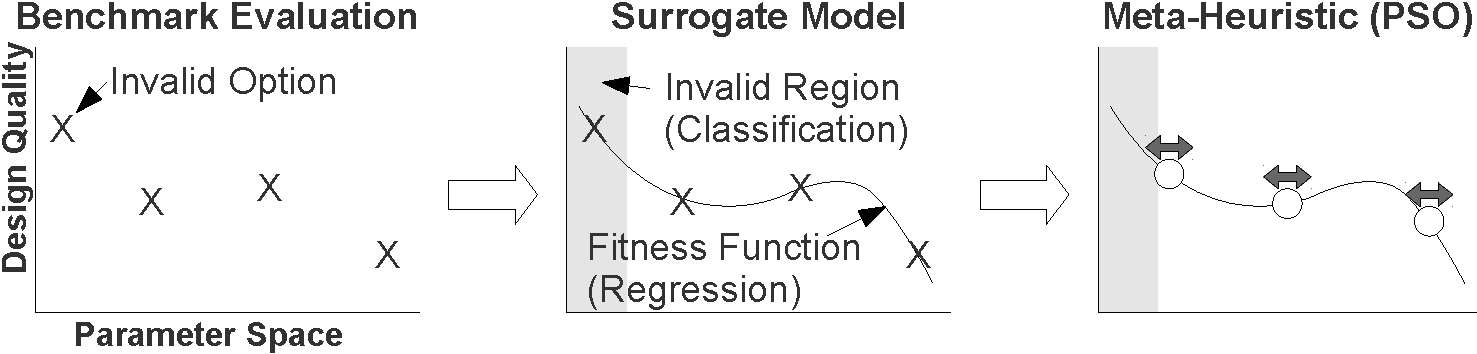
\includegraphics[width=1.0\textwidth]{./figs/surrogate_tobias.pdf}
        \caption{Benchmark evaluations, surrogate model and model guided search.}     
           \label{fig:ouridea}
  \end{figure*}
 
\subsubsection{\ac{alo} Surrogate Model}
\label{surrogatemodels}
%benchmark(x) = (metric(x) + ,t_i)\\
There are a few steps to build the surrogate model and use it to predict:
\begin{enumerate}\addtolength{\itemsep}{-0.1\baselineskip}  
\item Make use of Bayesian regressors to access the probability of prediction of $\hat{f}(\mathbf{x_*})$ of non-examined parameter configurations $\mathbf{x_*}$
\item Use classifiers to predict exit codes (valid or not) of $X_*$ across $\mathcal{X}$.
\item Predict the exit code and fitness value for a unknown parameter using both models.
\end{enumerate}

Admittedly, building surrogate model will also need a certain amount of effort by using a Bayesian regressor together with a classifier to create a novel surrogate model based on the given fitness function. However, it is worth doing since it will reduce substantial effort afterwards.

\subsubsection{Parameter Space} 
\label{designspace}
The parameter space $\mathcal{X}$ of a reconfigurable design is spanned by discrete and continuous parameters determining both the architecture and physical settings of \ac{fpga} designs \cite{arc2012MLO}. A vector $\mathbf{x}$ represents a parameter configuration within the parameter space $\mathcal{X} = \mathcal{X}_1 \times ... \times \mathcal{X}_D $ such that any $\mathcal{X}_{d} \subseteq \mathbb{R}$. We should notice that in the real problem of FPGA design, the parameter is either discrete or continuous, which make the design space more sophistic and as a consequence, several effort should be done to handle this well.

%\vspace{-0.5em}

%
%\subsection{\ac{alo} Algorithm}
%\label{aloalgo}

However, when there are more than one objective functions for optimizing, we should take all of the fitness functions into consideration when we do the meta-iteraration. Also, since there are multiple objectives, it's hard to find a 'best' particle which is both the best for all objectives. Instead, we wish to find trade-off between these objectives, thus the concept of \ac{moalo} arises. 


%\vspace{-0.5em}

%\vspace{-2.5em}
%
%\subsection{\ac{alo} termination criteria and usage scenario}
%\label{term}
\section{MOMLO}
\subsection{Objective Functions}
Multi-objective optimization problems occur in many different real-world domains and particularly in the FPGA design problem. Optimization problems that have more that one objective function are rather common in every field or area of knowledge. In such problems, the objectives to be optimized are normally in conflict with respect to each other, which means it is hard to find a single solution for all of these problems. Consider the following 4 scenarios for the FPGA design:
\begin{list}{$\bullet$}{\itemsep 0.5ex}
\item We evaluate our first configuration with the parameters $\vec{\mathbf{x}_1}$ in the FPGA architecture, it shows poor performance on both power consumption and accuracy, with a score of 54 and 70 on the evaluation measure respectively. 
\item Then evaluate one another configuration with the parameters $\vec{\mathbf{x}_2}$, it shows really good performance on the power consumption, say 20. Unfortunately it has a poor accuracy of only 68. 
\item After we evaluate one more configuration $\vec{\mathbf{x}_3}$ which shows good performance on the accuracy, say 39. Unfortunately it has a poor performance on the power consumption with 60 on the evaluation measure. 
\item At last we evaluate a slightly better configuration $\vec{\mathbf{x}_4}$ which has a power consumption of 42 and  accuracy of 48. 
\end{list}

From the above 4 scenarios, we would first declaim that the $\vec{\mathbf{x}_1}$ is poor on both power consumption and accuracy and therefore it is thrown away. When considering the next 3 designs, however, we cannot say which one is better than the rest because each of them has its own strength on one aspect. Therefore, the algorithm should return all of them and let the designers to decide which one to use.

To conclude, in multi-objective MLO we want to achieve a balanced solution for the FPGA design with respect to several objectives such as power, execution time or accuracy, etc.  Solving multi-objective optimization problems can be done in several ways and the one we use in this paper is the Multi-objective PSO.

In the multi-objective PSO, it is hard to find a global optimum and then we are now facing this problem:
\begin{align} 
\label{eq:mo1}
\mathbf{\min_x\overrightarrow{f_*(x)}}=[ f_1(\overrightarrow{x} ),f_2 (\overrightarrow{x} ),\ldots,f_k (\overrightarrow{x} ) ]
\end{align} 

where $ \mathbf{\overrightarrow{x}}=[x_1,x_2,\ldots,x_n] $ is the vector of decision variables, there are a total of k objectives, among which $\mathbf{f_i: \mathbb{R}^n \to \mathbb{R} }, i=1,2,...,k$ are the objective functions.

\begin{description}
  \item[Definition 1.] Given two vectors, $\mathbf{\overrightarrow{x}, \overrightarrow{y} \in \mathbb{R}^k}$, we say that $\overrightarrow{x} \leq \overrightarrow{y}$ if $x_i \leq y_i$ for $i = 1, \dots, k$, and that $\overrightarrow{x}$ $\mathbf{dominates}$  $\overrightarrow{y}$ (denoted by $\overrightarrow{x} \prec \overrightarrow{y}$ and $\overrightarrow{x} \neq \overrightarrow{y}$).
\\
  \item[Definition 2.] We say that a vector of parameters in parameter space of decision variables $\overrightarrow{x} \in \chi \subset \mathbb{R}^n$ is $\mathbf{non-dominated}$ with respect to $\chi$, if there does not exist another $\overrightarrow{x'} \in \chi$ such that $\overrightarrow{f(\overrightarrow{x'})} \prec  \overrightarrow{f(\overrightarrow{x})}$.
\\
  \item[Definition 3.] We say that a vector of decision variables $\overrightarrow{x*} \in \mathcal{D} \subset \mathbb{R}^n$ ($\mathcal{D}$ is the feasible region) is $\mathbf{Pareto-optimal}$ if it is non-dominated with respect to $\mathcal{D}$.
\\
 \item[Definition 4.] The $\mathbf{Pareto Optimal Set}$  $\mathcal{P}*$ is defined by:
\begin{center} 
$\mathcal{P}*$ = \{$\overrightarrow{x} \in \mathcal{D} | \overrightarrow{x}$ is Pareto-optimal\}
\end{center}

 \item[Definition 5.] The $\mathbf{Pareto Front}  \mathcal{PF}*$ is defined as:
\begin{center} 
$ \mathcal{PF}*= \{\overrightarrow{f}(\overrightarrow{x}) \in  \mathbb{R}^k | \overrightarrow{x} \in \mathcal{P}*\}$
\end{center}.
\end{description}

In such problems, the objectives to be optimized are normally in conflict with respect to each other, which indicates that there is no single solution for all of these problems. Instead, we aim to find "trade-off" solutions that achieves the best possible compromises among these objectives. In other words, we wish to find the Pareto Optimal Set $\mathcal{P}*$ which is an approximation of the Pareto Front $\mathcal{PF}*$ \cite{mosurvey}. 

\subsection{Literature Review}
Since the first proposed Multi-Objective Particle Swarm Optimizer (MOPSO) developed by Moore and Chapman in 1999 \cite{moore1999}, more than thirty different MOPSOs have been reported in the specialized literature and usually they are mainly classified as the following methods \cite{mosurvey}.

\begin{list}{$\bullet$}{\itemsep 0.5ex}

\item Aggregating approaches: combine (or "aggregate") all the objectives of the problem into a single one, then the multi-objective problem is simply transformed into a single-objective version \cite{ag1,ag2}. The drawback is obviously that it is hard to find a optimum coefficient to represent the different objectives.

\item Lexicographic ordering: Rank the objectives in order of their importance. The optimum solution is then obtained by minimizing the objective functions separately, starting with the most important one and proceeding according to the predefined order of importance of the objectives \cite{lo1}. Again, the drawback is obvious that the importance is hard to be measured and therefore the design lose its precision.

\item Sub-Population approaches: involve the use of several subpopulations as single-objective optimizers. Then, the subpopulations of the PSO explore the parameter space separately and somehow exchange information or recombine among themselves aiming to produce trade-offs among the different solutions \cite{sp1,sp2}. This solution is somehow better but still suffer the problem of balancing the importance of several objectives.

\item Pareto-based approaches: These approaches use leader selection techniques based on Pareto dominance and select as leaders to the particles that are non-dominated with respect to the swarm \cite{pb1,pb2,pb3,pb4,pb5}. This is currently best solution for the Multi-objective optimization, however, the leader selection and non-dominate retaining method should be chosen carefully in order to reach great performance. Nowadays, several variations of the leader selection scheme are proposed and most authors adopt additional information to select leaders (e.g., information provided by a density estimator) in order to avoid a random selection of a leader from the current set of non-dominated solutions.

\item Combined approaches: Combination of the solutions above \cite{cb1,cb2}.

\end{list}

\subsection{MOMLO Algorithm}

% pseudo code
\alglanguage{pseudocode}
\begin{algorithm}
\footnotesize

\caption{MOMLO}\label{momlo}
\begin{algorithmic}[1]
\For{$\mathbf{x_*} \in X_*$} 
	\For{$\mathbf{i} \in \mathbf{1,2,...,N}$}
		\State $\mathbf{x_*}.\overrightarrow{fit_i} \gets \overrightarrow{f_i}(\mathbf{x_*})$ \Comment{Initialize with a uniformly randomized set for every objectives $f_i*$ in the fitness function.}
	\EndFor
\EndFor
\Repeat   
  
    \For{$\mathbf{x_*} \in X_*$}
      \State $\overrightarrow{y_*},\rho_{max}  \gets$ $regressor(\mathcal{D}_{r},\mathbf{x_*})$
      \State $t_* \gets $ $classifier(\mathcal{D}_{c},\mathbf{x_*}$)
    	\If {$\rho_{max}  < min_{\rho}$ and $t_*=0$}
        	\State $\mathbf{x_*}$.$\overrightarrow{fit}$ $\gets \overrightarrow{y_*}$
      		\Else
       		 \If {$t_*=0$}
         		 \State $\mathbf{x_*}.\overrightarrow{fit} \gets$ $\overrightarrow{f(\mathbf{x_*}})$
	        \Else 
    		     \State $\mathbf{x_*}.\overrightarrow{fit} \gets \vec{\max_{val}}$ or $\vec{\min_{val}}$
	        \EndIf
    	\EndIf
    \EndFor
	\State $X_* \gets Meta(X_*)$ \Comment{Iteration of the meta-heuristic}
\Until{Termination Criteria Satisfied}  

\end{algorithmic}
\end{algorithm}

We present our \ac{moalo} in Algorithm~\ref{momlo}. The algorithm's main change for the previous \ac{alo} \cite{arc2012MLO} is the fitness function now return a vector $\overrightarrow{f_i}$ of fitness values and as a result, the model is trained for each fitness values.  We initialize the meta-heuristic of our choice with $N$ particles $X_*$ uniformly randomly scattered across $\mathcal{X}$. Each particle has an associated fitness vector $\mathbf{x}.\overrightarrow{fit}$ and a position $\mathbf{x}$. Now after training the models, the predictor now get a vector of output for the prediction of each fitness functions as well as the variance. For simplicity, we only retain one variance which is the biggest value $\rho_{max}$ after the prediction and the further judgement on how good the fitness vector is fully based on this single value. Similarly, for the predict code from the classifier, a vector of predictions from all the objective models is simplified by only one value $t_*$( any $t_i = 1$ means the model prediction is invalid). For all $\mathbf{x_*}$ predicted to lie in $\mathcal{V}$ we proceed as follows. Whenever $\rho$ returned by the regressor is smaller than the minimum required confidence $min_{\rho}$ we use the $y_*$; otherwise we assume the prediction to be inaccurate and evaluate $f(\mathbf{x_*})$. The meta-heuristic will avoid $\mathcal{I}$ and $\mathcal{F}$ regions as they are both assigned unfavorable $\vec{\max_{val}}$ or $\vec{\max_{val}}$ vectors in respect to the fitness functions. We construct the training sets $\mathcal{D}_{c}$ and $\mathcal{D}_{r}$ as described in Algorithm~\ref{momlo}. Whenever $b(\mathbf{x_*})$ is evaluated,  $(\mathbf{x_*},t_*)$ is included within the classifier training set $\mathcal{D}_{c}$. If exit code is valid ($t_*=0$), then $(\mathbf{x_*},y_*)$ is added to $\mathcal{D}_{r}$. 

In order to apply the meta-heuristic strategy for solving multi-objective optimization problems of the FPGA, it is obvious that the original scheme has to be modified. As we saw in Section II, the solution set of a problem with multiple objectives does not consist of a single solution (as in global optimization). Instead, in multi-objective optimization, we aim to find a set of different solutions (the so-called Pareto Optimal Set $\mathcal{P}*$) in order to have a better approximation of the Pareto Front. 
The pseudo code is defined as follows, First, the swarm is initialized. This initialization includes both positions and velocities. The corresponding $pbest$ of each particle is initialized and the leader is located (usually the $gbest$ solution is selected as the leader). Then, for a maximum number of iterations, each particle flies through the search space updating its position (using (4) and (5)) and its $pbest$ and, finally, the leader is updated too.
\alglanguage{pseudocode}
\begin{algorithm}
\footnotesize

\caption{MOPSO}\label{ourmlo}
\begin{algorithmic}[1]
	\State Initialize swarm
	\State Initialize leaders in an external archive
	\State $g \gets 0$
	\While{$i \leq 10$}
            \For {$ particle \in Population $}  
		\State Select leader
		\State Update Position (Flight)
		\State Mutation
		\State Evaluation
		\State Update $pbest$

	   \EndFor
		\State Update leaders in the external archive
		\State Quality(leaders)
		\State $g \gets g+1$
	\EndWhile
	\State Report Pareto Front in the external archive
\end{algorithmic}
\end{algorithm}

In fact, the criterion of how good a Pareto Optimal Set $\mathcal{P}*$ varies a lot since there is no global best to be measured. In general, when solving a multi-objective problem, three are the main goals to achieve \cite{mocompare}:

\begin{list}{$\bullet$}{\itemsep 0.6ex}

\item Maximize the number of elements of the Pareto Optimal Set $\mathcal{P}*$ found.
\item Minimize the distance of the individuals Pareto Optimal Set $\mathcal{P}*$ produced by our algorithm with respect to the true (global) Pareto Optimal Set $\mathcal{P}*$ (assuming we know its location).
\item Maximize the spread of solutions found, so that we can have a distribution of vectors as smooth and uniform as possible.


\end{list}

Given the population-based nature of PSO, it is desirable to produce several (different) non-dominated solutions with a single run. So, as with any other evolutionary algorithm, the three main issues to be considered when extending PSO to multi-objective optimization are \cite{moissue}:
\begin{list}{$\bullet$}{\itemsep 0.6ex}

\item How to select leaders for each particle to guide the particle to find non-dominated solution and then have a better approximation on the Pareto Front?
\item How to give a criterion on whether to retain a non-dominated solution to the Pareto Optimal Set $\mathcal{P}*$, which means the found solutions should be well spread along the Pareto Front and the total amount of which should be restricted on a reasonable limit. 
\item How to maintain diversity in the swarm in order to avoid premature convergence to a single solution?
\end{list}
For our version of Multi-Objective MLO, we design carefully in respect of the performance and feasibility of different method that have proposed by the others. Since we have two criterions to select the method: 


\begin{list}{$\bullet$}{\itemsep 0.6ex}
\item The method should give good performance on selection and updating of leaders as well as creation of new solutions.
\item It must be easy implemented and compatible for our previous solution.
\end{list}

% new section
\section{Design} 
\label{design}
\subsection{Leaders in Multi-Objective Optimization}
Although a few researches have avoided the problem of defining a new concept of leader for multi-objective problems by adopting aggregating functions (i.e., weighted sums of the objectives) or approaches that optimize each objective separately \cite{mosurvey}, they are not suitable for the FPGA design since the weight of the different objectives vary a lot on different FPGA applications.

In our solution, the different objectives are controlled by the weights but they are only for the flight of the particles. In this way, a quality measure that indicates how good is a leader is very important. Obviously, such feature can be defined in several different ways. One possible way of defining such quality measure can be related to density measures. Promoting diversity may be done through this process by means of mechanisms based on some quality measures that indicate the closeness of the particles within the swarm.
Nearest neighbor density estimator \cite{nsga2002}. The nearest neighbor density estimator gives us an idea of how crowded are the closest neighbors of a given particle, in objective function space.
\begin{figure}
\centering
\begin{tikzpicture}[x=1.4cm,y=1.4cm]

  \def\xmin{0}
  \def\xmax{5}
  \def\ymin{0}
  \def\ymax{5}


  % axes
  \draw[-latex,line width = 2pt] (\xmin,\ymin) -- (\xmax,\ymin) node[right] {\LARGE $f_1$};
  \draw[-latex,line width = 2pt] (\xmin,\ymin) -- (\xmin,\ymax) node[above] {\LARGE $f_2$};


\draw[dotted]
    (4.4,0.4) node[circle,fill = black, inner sep=2pt] {}
    (3.7,0.7) node[circle,fill = black, inner sep=2pt] {}
   (3.2,0.9) node[circle,fill = black, inner sep=2pt] {}
   (3.2,0.9) node[above right=2pt] {\LARGE i+1} 
   (1.8,2) node[circle,fill = black, inner sep=2pt] {}
   (1.8,2) node[above right=2pt] {\LARGE i-1} 
   (2.5,1.4) node[circle,fill = black, inner sep=2pt] {}
   (2.5,1.4) node[above right=2pt] {\LARGE i} 
   ( 0.9,3.0) node[circle,fill = black, inner sep=2pt] {}
(1.4,2.4) node[circle,fill = black, inner sep=2pt] {}
(0.5,3.6) node[circle,fill = black, inner sep=2pt] {};

\draw[dashed] (1.8,2) -- (2.5,1.4);
\draw[dashed] (2.5,1.4) -- (3.2,0.9);

\end{tikzpicture}
\caption{The neighbor density estimator for and example with two objective functions. Particles with a large distance from the neighbors is preferred.}
\end{figure}

\subsection{Retaining and Spreading Non-dominated Solutions}
As we mentioned before, it is important to retain the non-dominated solutions found along all the search process so that we can report at the end those solutions that are non-dominated with respect to all the previous populations. 

The most straightforward way of retaining solutions that are non-dominated with respect to all the previous populations (or swarms) is to use an external archive \cite{mosurvey}. Such an archive will allow the entrance of a candidate solution only if: (a) it is non-dominated with respect to the current stored solution in the archive or (b) it dominates any of the solutions within the archive (in this case, the dominated solutions have to be deleted from the archive) \cite{mosurvey}. This approach has, however, the drawback of increasing the size of the archive exponentially. 

Recently, other researchers have proposed the use of relaxed forms of dominance. The main one adopted in PSO has been "$\epsilon$-dominance" \cite{epsilon2002}, which concept is illustrated in the definitions 6 \cite{epsilon2003}. The $\epsilon$-dominance solution is believed to be able to generate well-formed Pareto Optimal Set as well as perform a much quicker converge speed.
\begin{description}
\item [Definition 6($\epsilon$- Dominance)]: 
Let $\mathnormal{f,g} \in \mathbb{R}^m$. Then  $\mathnormal{f}$ is said to $\epsilon- dominante$ $ \mathnormal{g}$ for some $\epsilon > 0$, denoted as $\mathnormal{f} \succ_\epsilon \mathnormal{g}$, iff for all $i \in \{1, \dots, m\}$ 

\begin{align} 
\label{eq:edominate1}
(1+\epsilon)\cdot  \mathnormal{f}_i  \geq \mathnormal{g}_i. 
\end{align} 

\end{description}

\begin{figure}
\centering
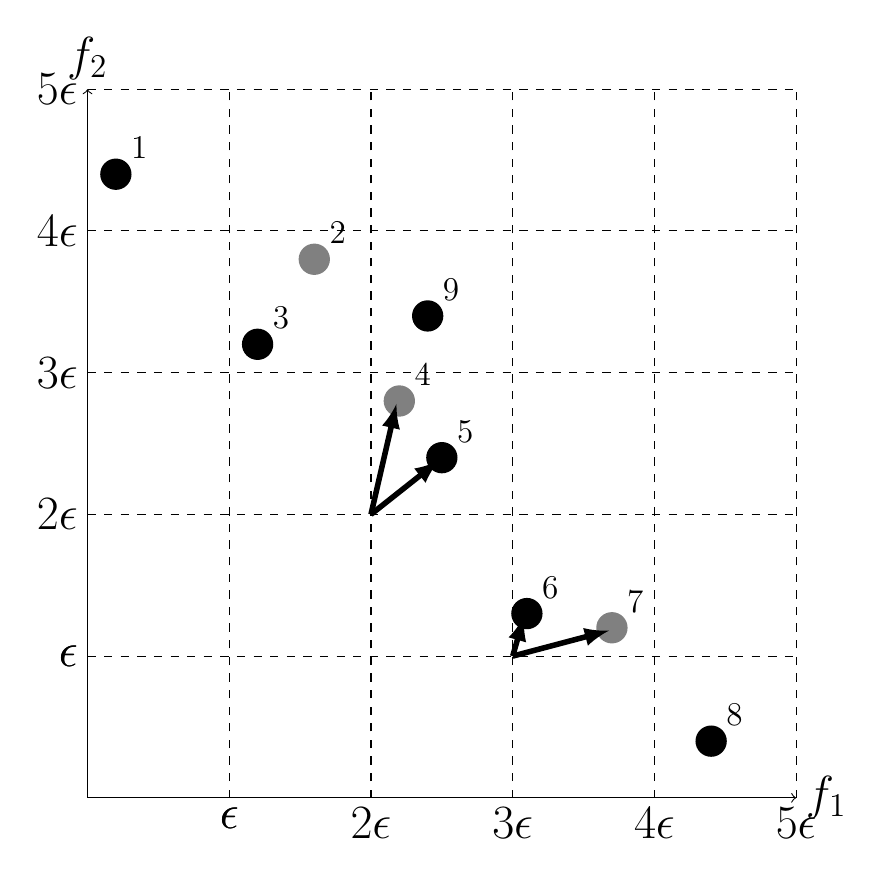
\begin{tikzpicture}[x=1.8cm,y=1.8cm]

  \def\xmin{0}
  \def\xmax{5}
  \def\ymin{0}
  \def\ymax{5}

  % grid
  \draw[style=dashed, ystep=1, xstep=1] (\xmin,\ymin) grid
  (\xmax,\ymax);

  % axes
  \draw[->] (\xmin,\ymin) -- (\xmax,\ymin) node[right] {\LARGE $f_1$};
  \draw[->] (\xmin,\ymin) -- (\xmin,\ymax) node[above] {\LARGE $f_2$};

  % xticks and yticks
  \foreach \x in {,,2,3,4,5}
    \node at (\x, \ymin) [below] {\LARGE \x$\epsilon$};
  \foreach \y in {,,2,3,4,5}
    \node at (\xmin,\y) [left] {\LARGE \y$\epsilon$};

% draw the dotted
\draw[dotted]
    (2.4,3.4) node[circle,fill = black, inner sep=4pt] {}
    (2.4,3.4) node[above right=2pt] {\large 9} 
    (4.4,0.4) node[circle,fill = black, inner sep=4pt] {}
    (4.4,0.4) node[above right=2pt] {\large 8} 
    (3.7,1.2) node[circle,fill = gray, inner sep=4pt] {}
(3.7,1.2) node[above right=2pt] {\large 7} 
   (3.1,1.3) node[circle,fill = black, inner sep=4pt] {}
(3.1,1.3) node[above right=2pt] {\large 6} 
   (2.2,2.8) node[circle,fill = gray, inner sep=4pt] {}
   (2.2,2.8) node[above right=2pt] {\large 4} 
   (2.5,2.4) node[circle,fill = black, inner sep=4pt] {}
   (2.5,2.4) node[above right=2pt] {\large 5} 
   ( 1.2,3.2) node[circle,fill = black, inner sep=4pt] {}
( 1.2,3.2) node[above right=2pt] {\large 3} 
(1.6,3.8) node[circle,fill = gray, inner sep=4pt] {}
(1.6,3.8) node[above right=2pt] {\large 2} 
(0.2,4.4) node[circle,fill = black, inner sep=4pt] {}
(0.2,4.4) node[above right=2pt] {\large 1};

\draw [-latex,line width = 2pt] (2,2) -- (2.18,2.78);
\draw [-latex,line width = 2pt] (2,2) -- (2.48,2.38);
\draw [-latex,line width = 2pt] (3,1) -- (3.68,1.18);
\draw [-latex,line width = 2pt] (3,1) -- (3.08,1.28);
\end{tikzpicture}
\caption{A example of the use of $\epsilon$-dominance in an external archive. Solution 3 dominates solution 2, therefore solution 1 is preferred. Solutions 4 and 5 are incomparable. However, solution 5 is preferred over solution 4, since solution 5 is closer to the lower lefthand corner represented by point ($2\epsilon$, 2$\epsilon$).Solution 6 is preferred compared to solution 7 for the same reason. Solution 9 is not accepted since its box, represented by point ($2\epsilon$, 3$\epsilon$) is dominated by the left box.}
\end{figure}

The main use of this concept in multi-objective PSO has been to filter solutions in the external archive. Mostaghim and Teich \cite{epsilon2003} have found that when comparing "$\epsilon$-dominance" against existing clustering techniques for fixing the archive size, the "$\epsilon$-dominance" method can find solutions much faster (computationally speaking) than the clustering technique with a comparable (and even better in some cases) convergence and diversity.

\subsection{Promoting Diversity while Creating New Solutions}
It is well known that one of the most important features of the PSO algorithm is its ability to find global optimum instead of blocked at a local one.This is a positive feature as long as we don't have premature convergence (i.e., convergence to a local optimum). Premature convergence is caused by the rapid loss of diversity within the swarm. When adopting PSO for solving multi-objective optimization problems, it is possible to promote diversity through the selection of leaders. 
In this way, we choose to use a mutation operator to help the flight of the particle is very important in order to escape from local optima and to improve the exploratory capabilities of PSO. 


\section{Implementation}
\label{Implementation}
As I illustrated in the previous part, there are 5 most important  functionalities to be implemented in order to maintain the Pareto Optimal Set:

\begin{list}{$\bullet$}{\itemsep 0.5ex}
\item Initialize the population of the particle swarm; 
\item Retrieve best global leader for each of the particles before it update its position;
\item Measure the density of a new found non-domininate particle;
\item Retain the new non-dominated solution based on the new fitness values;
\item Remove dominated solution from Pareto Optimal Set $\mathcal{P}*$;
\end{list}


\subsection{Initialize}
\begin{list}{$\bullet$}{\itemsep 0.5ex}

\item At first we create an empty Pareto Optimal Set dictionary $\mathcal{P}*$, set the size of the Dictionary as the maximum amount of Pareto Optimal Set points we want. Every entry of the $\mathcal{P}*$ is another dictionary including the particle's position and fitness values.
\item Then for every initialized particle in the population, evaluate the fitness tuple $\mathcal{T}$ using the multi-objective fitness function.
\item Check if this $\mathcal{T}$ dominate every points in the Pareto Set $\mathcal{P}*$ and decide whether to store this fitness tuple $\mathcal{T}$ into the external Pareto Optimal Set $\mathcal{P}*$ or not.
\item Retrieve the Pareto Optimal Set $\mathcal{P}*$ and assign a leader for every particle.
\end{list}

\subsection{Retrieve}

   For every Pareto Point in the Pareto Optimal Set $\mathcal{P}*$, a nearest neighbor density (crowding radius) estimator is chosen to maintain it's suitability as leader and thus to promote diversity. Three methods have been implemented to select leader based on this density measure.

\begin{list}{$\bullet$}{\itemsep 0.5ex}
\item Choose the Least density particle (one has the $density_{min}$): For every member of Pareto non-dominate particles (stored in a external achieve), a neighbor density is computed and then chooses the least density one.
\item By means of Tournament: For every member of Pareto non-dominate particles (stored in an external achieve), a neighbor density is computed and then the top $k$ (usually a small positive integer) particles are chosen then select one randomly within them.
\item By means of a Roulette selection: That is for every member of Pareto non-dominate particles (stored in a external achieve), a neighbor density is computed and then chooses it with roulette. A particle with a small neighbor density has more probability to be chosen since the neighbor is less density. 
\end{list}

\subsection{Neighbor Density Estimator}
Euclidean Distance is chosen as the measure of each two particles in the Pareto Optimal Set achieve, however, there still remaining one question that how we represent the distance for a particle in the Pareto Optimal Set $\mathcal{P}*$, namely the neighbor density. Two methods are implemented to calculate the neighbor density. 

\begin{list}{$\bullet$}{\itemsep 0.6ex}
\item Nearest $k$ neighbors: That is for every member of Pareto non-dominate particles (stored in a external achieve), a Euclidean distance is computed between it and every others and then bottom $k$ with less distance than others are chosen to add up as the neighbor density. In my program the k is set to be 2, namely to calculate it's nearest two neighbors (left one and right one in 2-D space).
\item Niche neighbors: That is for every member of Pareto non-dominate particles (stored in a external achieve), a Euclidean distance is computed between it and every others, and then only the ones within that niche count are retained to add up as the neighbor density. The size of niche may influence the result a lot, so it should be carefully chosen for each run.
\end{list}

\subsection{Retain}
Every time when a non-dominated solution is discovered, a new question raise for whether it should be added to the Pareto Optimal Set $\mathcal{P}*$ as discussed in the previous part to prevent premature converge and over-sized achieve. Two methods are implemented to calculate the neighbor density. 

\begin{list}{$\bullet$}{\itemsep 0.6ex}
\item Simple Retain with replacement: After the non-dominated property of the given particle has been proved, the particle is treated as a candidate for entering the Pareto Optimal Set $\mathcal{P}*$. If the set is not full (the size is set by the configuration), the particle gets its right to be retained. However, if the $\mathcal{P}*$ is full, the most density one (computed by the previous density measure) has to be replace by this new particle or the new particle won't be able to be retained.
\item $\epsilon$-dominate retain measure: In this case, the simple dominate property won't be enough for the particle to be retained. After the simple non-dominated property of the given particle has been proved, the particle is again treated as a candidate for entering the Pareto Optimal Set $\mathcal{P}*$. Then as discussed in previous part, the Pareto Optimal Set $\mathcal{P}*$ is divided to $\epsilon$ boxes, the one in the bottom left of each box is the implicit non-dominate point in this box. Then if the particle belongs to a certain box and the box is empty, it can be retained without competing. Otherwise, if a particle already exists in this particle, the candidate should compete with this particle, if one of the two wins, it will be retained and if both of them cannot dominate each other, the one near the implicit non-dominate point in the bottom left will be chosen.
Again, the value of $\epsilon$ should be carefully chosen as it may place a tremendous influence on the result. In my implementation, $\epsilon$ starts with a minimal $\epsilon$ = 0.0075, which is systematically increased every time the number of archived vectors exceeds a predetermined maximum size. 
\end{list}

\subsection{Auxiliary Functionalities}
\begin{list}{$\bullet$}{\itemsep 0.6ex}
\item Fitness Values Tuple $\mathcal{T}$: For the multi-objective optimization problem, the fitness is no longer one value but a tuple of the values from different fitness values. Thus the existing data structure for the particle fitness should be change to tuples ($f_1$, $f_2$, $\dots$, $f_n$).

\item Train and Predict: Each objective has its own fitness function, so does the surrogate model. In the problem of multi-objective optimization, the number of models equals to the number of objective functions. During the implementation, the training functions train surrogate model for every fitness functions and then a list of models are stored instead of just one model. The predict procedure are almost the same, however, some more implementation should be done since there are a list of results from different models. For the final result, only the predictions of the different fitness values should be retained in a tuple but the classification and variances should be only one value or a vector ($t_{t_i = 0}$ and $\rho_{max} $) in respect to the parameter space  $\mathcal{X}$. 

\item Non-dominate Criterion: The non-dominate property of each particle is simple and which can be specialized for every maximization/minimization problem. For every single fitness function in the multi-objective optimization, the particle should give better performance than others and this particle is defined dominate others. However, if only one fitness value is not better, it cannot dominate the others and if it has at least one fitness value is better, it is a non-dominated point.

\item Termination Condition: The Termination Condition now is different from the single-objective one, that is there is no best fitness value we can decide as the termination condition like we do in the single objective one. Now other than the generation budget and number of times we evaluate the fitness functions, another criterion on how good the Pareto Optimal Set  $\mathcal{P}*$ is has been implemented: when the Pareto Optimal Set  $\mathcal{P}*$ has reach the size we pre-defined in the configuration, a variance value of them is computed and if the variance is well below a predefined criterion. In that condition, it is believed that the Pareto Optimal Set is an appropriate approximation of the Pareto Optimal Set.


\item Multi-objective Plot function: The plot function for multi-objective one is again different since now a few of fitness functions should be shown and the same as the surrogate models and most importantly, the Pareto Optimal Set. 

\end{list}
The main concepts behind the original MLO and the mutli-objective version are the same and as such we are not going to present them.

\section{Evaluation}
\label{evaluation}

The evaluation takes on four different  multi-objective functions by combining the artificial continuous functions provided by deap evolutionary algorithm package in python(See Fig.~\ref{fig:fitexample} for examples):
\begin{enumerate}\addtolength{\itemsep}{0.2\baselineskip}  
\item Two single-objective functions (minimizaiton functions): sphere and schaffer, see table~\ref{tab:f1} for details of the functions.
\item Two single-objective functions (maximizaiton functions): sphere and rastrigin, see table~\ref{tab:f2}.
\item One bi-objective function (minimizaiton functions):  fonseca, see table~\ref{tab:f3}
\item Three-objective function (minimizaiton functions): One single objective function (sphere) and one bi-objective function (fonseca), see table~\ref{tab:f4}.
\end{enumerate}

\begin{figure}
        \centering
        \begin{subfigure}[b]{0.35 \textwidth}
                \centering
                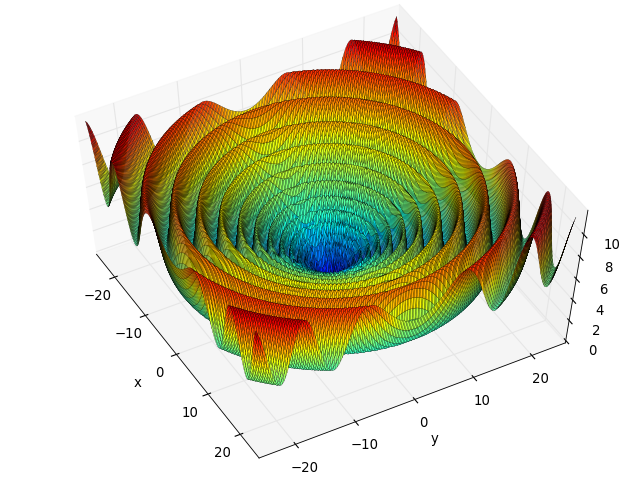
\includegraphics[width=\textwidth]{./figs/schaffer.png}
                \subcaption{schaffer}
        \end{subfigure}
        \begin{subfigure}[b]{0.35 \textwidth}
                \centering
                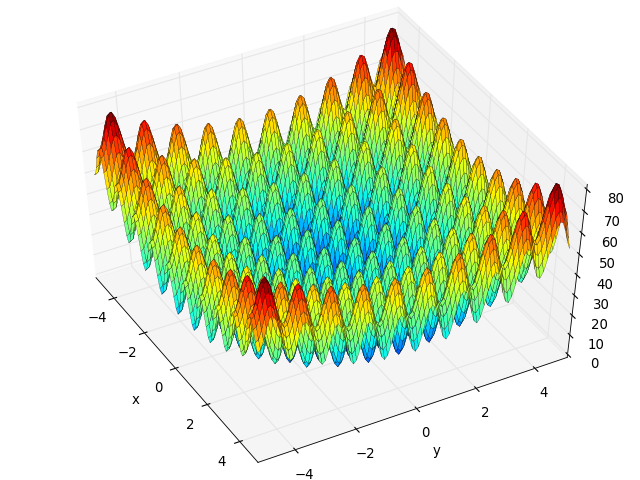
\includegraphics[width=\textwidth]{./figs/rastrigin.png}
                \subcaption{rastrigin}
        \end{subfigure}
        \caption{Single-objective artificial continious examples.}\label{fig:fitexample}
\end{figure}


\begin{table}
  \caption{Multi-objective function 1}  
  \label{tab:f1}
    \begin{center}
\begin{tabular}{c|c|ccc} 
\toprule 
 %&  \multicolumn{3}{c}{$\epsilon_{rms}$ } \\
	$\mathbf{Attributes}$ & $\mathbf{Function 1: sphere}$ & $\mathbf{Function 2: schaffer}$\\
	\hline Type & minimization & minimization \\
	Range & none & $x \in [-100,100]$\\ 
         Global optima & $x_i = 0, \forall x \in \{1,...,X\}, f(x) = 0$ & $x_i = 0, \forall x \in \{1,...,X\}, f(x) = 0$\\
         Function & $f(x) = \sum_{i=1}^{N} x_i^2$&$f(x) = \sum_{i=1}^{N-1} (x_i^2+x_{i+1}^2)^{0.25}\cdot\sin^2(50\cdot(x_i^2+x_{i+1}^2)^{0.1}+1) $\\
\bottomrule 
\end{tabular} 
\end{center}
\end{table}

\begin{table}
  \caption{Multi-objective function 2}  
  \label{tab:f2}
    \begin{center}
\begin{tabular}{c|c|ccc} 
\toprule 
 %&  \multicolumn{3}{c}{$\epsilon_{rms}$ } \\
	 $\mathbf{Attributes}$ & $\mathbf{Function 1: sphere}$ & $\mathbf{Function 2: rastrigin}$\\
	\hline Type & maximization & maximization\\
	Range & none & $x \in [-5.12,5.12]$\\ 
         Global optima & $x_i = 0, \forall x \in \{1,...,X\}, f(x) = 0$ & $x_i = 0, \forall x \in \{1,...,X\}, f(x) = 0$\\
         Function & $f(x) = \sum_{i=1}^{N} x_i^2$&$f(x) = 10N\sum_{i=1}^N x_i^2-10\cos{(2\pi x_i)} $\\
\bottomrule 
\end{tabular} 
\end{center}
\end{table}



\begin{table}
  \caption{Multi-objective function 3}  
  \label{tab:f3}
    \begin{center}
\begin{tabular}{c|cccc} 
\toprule 
 %&  \multicolumn{3}{c}{$\epsilon_{rms}$ } \\
	$\mathbf{Objectives}$ & $\mathbf{fonseca\ multi-objective\ function}$\\
	\hline Function 1& $f_{Fonseca1}(\vec{x})=1-e^{-\sum_{i=1}^3 (x_i - \frac{1}{\sqrt{3}}} )$\\
	Function 2&$ f_{Fonseca2}(\vec{x})=1-e^{-\sum_{i=1}^3 (x_i + \frac{1}{\sqrt{3}}} )$\\
\bottomrule 
\end{tabular} 
\end{center}
\end{table}
\begin{table}
  \caption{Multi-objective function 4}  
  \label{tab:f4}
    \begin{center}
\begin{tabular}{c|cccc} 
\toprule 
 %&  \multicolumn{3}{c}{$\epsilon_{rms}$ } \\
	 $\mathbf{Objectives}$ & $\mathbf{fonseca\ multi-objective\ function}$\\
	\hline Function 1& $f(x) = \sum_{i=1}^{N} x_i^2$\\
	Function 2& $f_{Fonseca1}(\vec{x})=1-e^{-\sum_{i=1}^3 (x_i - \frac{1}{\sqrt{3}}} )$\\
	Function 3& $ f_{Fonseca2}(\vec{x})=1-e^{-\sum_{i=1}^3 (x_i + \frac{1}{\sqrt{3}}} )$\\
\bottomrule 
\end{tabular} 
\end{center}
\end{table}



In all runs of the examples, we use \acp{gp} utilizing an isotropic exponential kernel with additive Gaussian noise. We choose \acp{svm} as our classifier with a \ac{rbf} kernel. Due to its simplicity and effectiveness we use a velocity clamping version of \ac{pso} with $c_1$ and $c_2$ set to 2.0. All presented results are averaged over 10 trials. 

Additionally, For the purpose of evaluating the performance on different approaches to select leaders and retain non-dominate point in the \ac{mopso}, we run a series of trials based on the same fitness function with different approaches and give comparison by providing the graphs of Pareto Front $\mathcal{PF}$ and tracing the velocity of the particles.




%\subsection{Artificial Benchmarks}
%\label{artbench}
%To verify \ac{alo} we use the standard meta-heuristic benchmark functions, especially $f$ evaluation limiting mechanisms. The functions are defined over continuous space and we use the results to compare \ac{alo} to alternative algorithms which are only defined in $\mathbb{R}^n$. The application settings are; $N=20$, $max_{std}=0.01$, $max_{iter}=10,000$, $F=10$, and $M=500$. $\mathcal{X}$ is limited to $[-2.0,2.0]^2$. All of the functions are smooth and F3. is periodic. The classification mechanism has no impact on the performance in this case, as the whole region of $\mathcal{X}$ is valid. We ran the benchmarks with a set of $M$ parameter, and the performance is similar to what is presented in Tab. \ref{tab:compschemes}, as long as $M$ is in the range of 100 and $max_{iter}$ is around $max_{eval}$ times larger. For lower $M$ the performance of \ac{alo} is still favorable. The fitness functions we used optimized are presented in Eq. \ref{eq:fitnessart}-\ref{eq:fitnessartlast}. The algorithm decreases the amount of fitness function evaluations by up to 80\% compared to \cite{5194095}. 
%
%\begin{align} 
%\label{eq:fitnessart}
%F1: f(x) =\sum_{i=1}^{n}{{x_{i}^{2}}} \\
%F2: f(x) =\sum_{i=1}^{n}{100{({x_{i+1}-x_{i}^{2}})}^{2} - {(1-x_{i})}^{2}} \\
%\label{eq:fitnessartlast}
%F3: f(x) ={ 1 \over 4000}\sum_{i=1}^{n}{{x_{i}^{2}}} - \prod_{i=1}^{n}{\cos{x_{i} / \sqrt{i}} + 1}
%\end{align}
%
% \begin{table}
%  \caption {Comparison of Surrogate Optimization Schemes.}  
%  \label{tab:compschemes}
%    \begin{center}
%\begin{tabular}{c c c}
%\toprule Function & GP-PSO \cite{5194095} & \ac{alo} \\ 
%\hline \textbf{F1} & 55 & 12 \\ 
% \textbf{F2} & 68 & 52 \\ 
% \textbf{F3} & 45 & 20 \\ 
%\bottomrule
%\end{tabular} 
%\end{center}
%\end{table}

%\begin{table*}
%\begin{tabular}{|c|c|c|c|c|c|c|c|c|c|c|c|}
%\hline p[kB] & slices & size & fmax & tp,e & tp & tr & tr,e &  ttotal[ms] & tr[ms] & tr,e[ms] & ttotal[ms] \\
%\hline 112 & 6921 & 404.1 & 250 & 4.0 & 4.00 & 80.8 & 0.72 & 80.9 & 1.347 & 0.012 & 1.39 \\
%\hline 56 & 3719 & 216.5 & 251 & 3.99 & 7.97 & 43.3 & 0.77 & 43.4 & 0.722 & 0.013 & 0.80 \\
%\hline 28& 2111 & 122.7 & 256 & 3.91 & 15.63 & 24.5 & 0.88 & 24.7 & 0.409 & 0.015 & 0.57 \\
%\hline 14& 1326 & 79.4 & 260 & 3.85 & 30.77 & 15.9 & 1.13 & 16.2 & 0.265 & 0.019 & 0.57 \\
%\hline 8 & 873 & 50.5 & 264 & 3.79 & 53.03 & 10.1 & 1.26 & 10.6 & 0.168 & 0.021 & 0.70 \\
%\hline 4 & 462 & 28.9 & 263 & 3.80 & 106.56 & 5.8 & 1.44 & 6.8 & 0.096 & 0.024 & 1.16 \\
%\hline 
%\end{tabular} 
%\caption{Table }
%\end{table*}

%\vspace{-1em}
%\vspace{-3.em}

\subsection{Results}
The results for all of the four different evaluations are plotted by the view function of \ac{moalo} ( Fig.~\ref{fig:shron}, Fig.~\ref{fig:max}, Fig.~\ref{fig:fonseca} and Fig.~\ref{fig:3d}). For each image: 
\begin{list}{$\bullet$}{\itemsep 0.4ex}
\item The top-left is the display of the Pareto Optimal Set $\mathcal{P}$;
\item The right two of it are the view of original fitness function and the two below them are the corresponding training models by the Gaussian regressors (the view may seen a little bit different from the original one because the models from regressors currently are not work perfectly especially for complicated fitness functions: it only can draw a sketch of the fitness function but not accuracy enough as the original one);
\item The lower two under them are the view of the design space (the green cross shows the original sample place for the particles and the white circles are the particles' position after the algorithm terminates) and the bottom-left sub-image is a plot of the average particle velocity within the current generations.
\end{list}

\begin{figure}
        \centering
    \centering
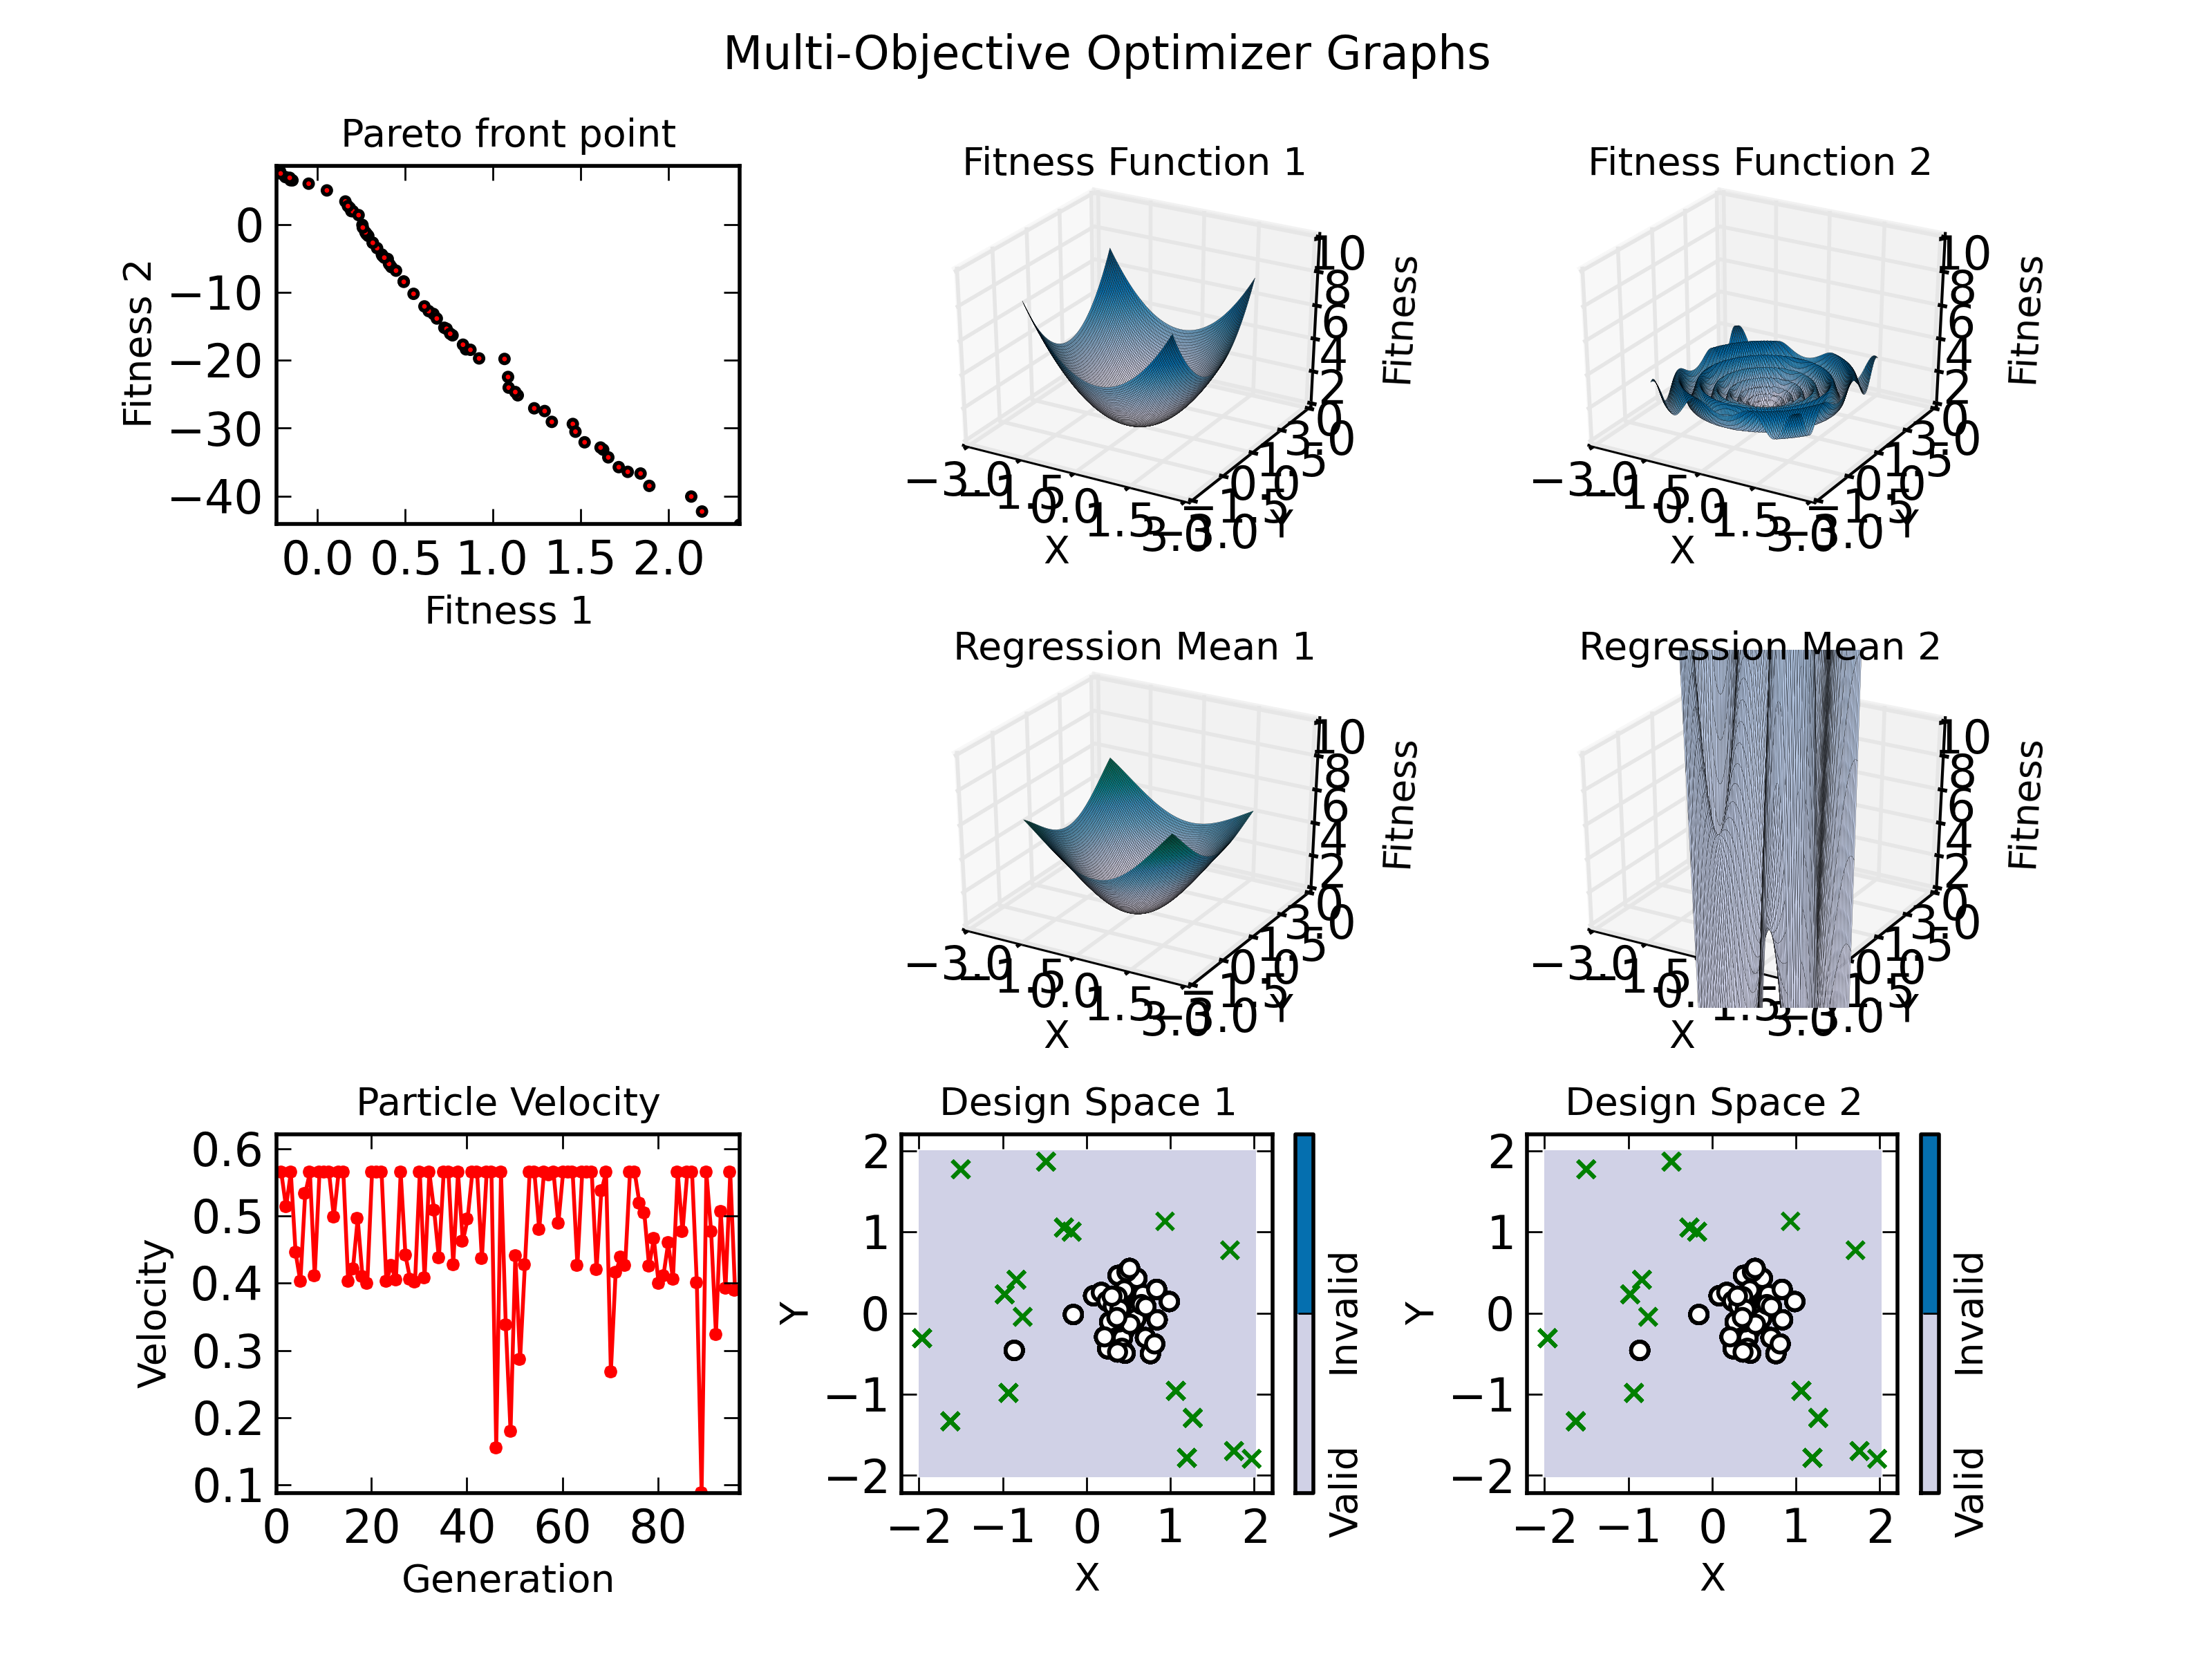
\includegraphics[width=0.8\textwidth]{./figs/shron.png}
        \caption{Plot of the run results image for two minimization single-objective artificial continious functions.}\label{fig:shron}
\end{figure}

\begin{figure}
        \centering
    \centering
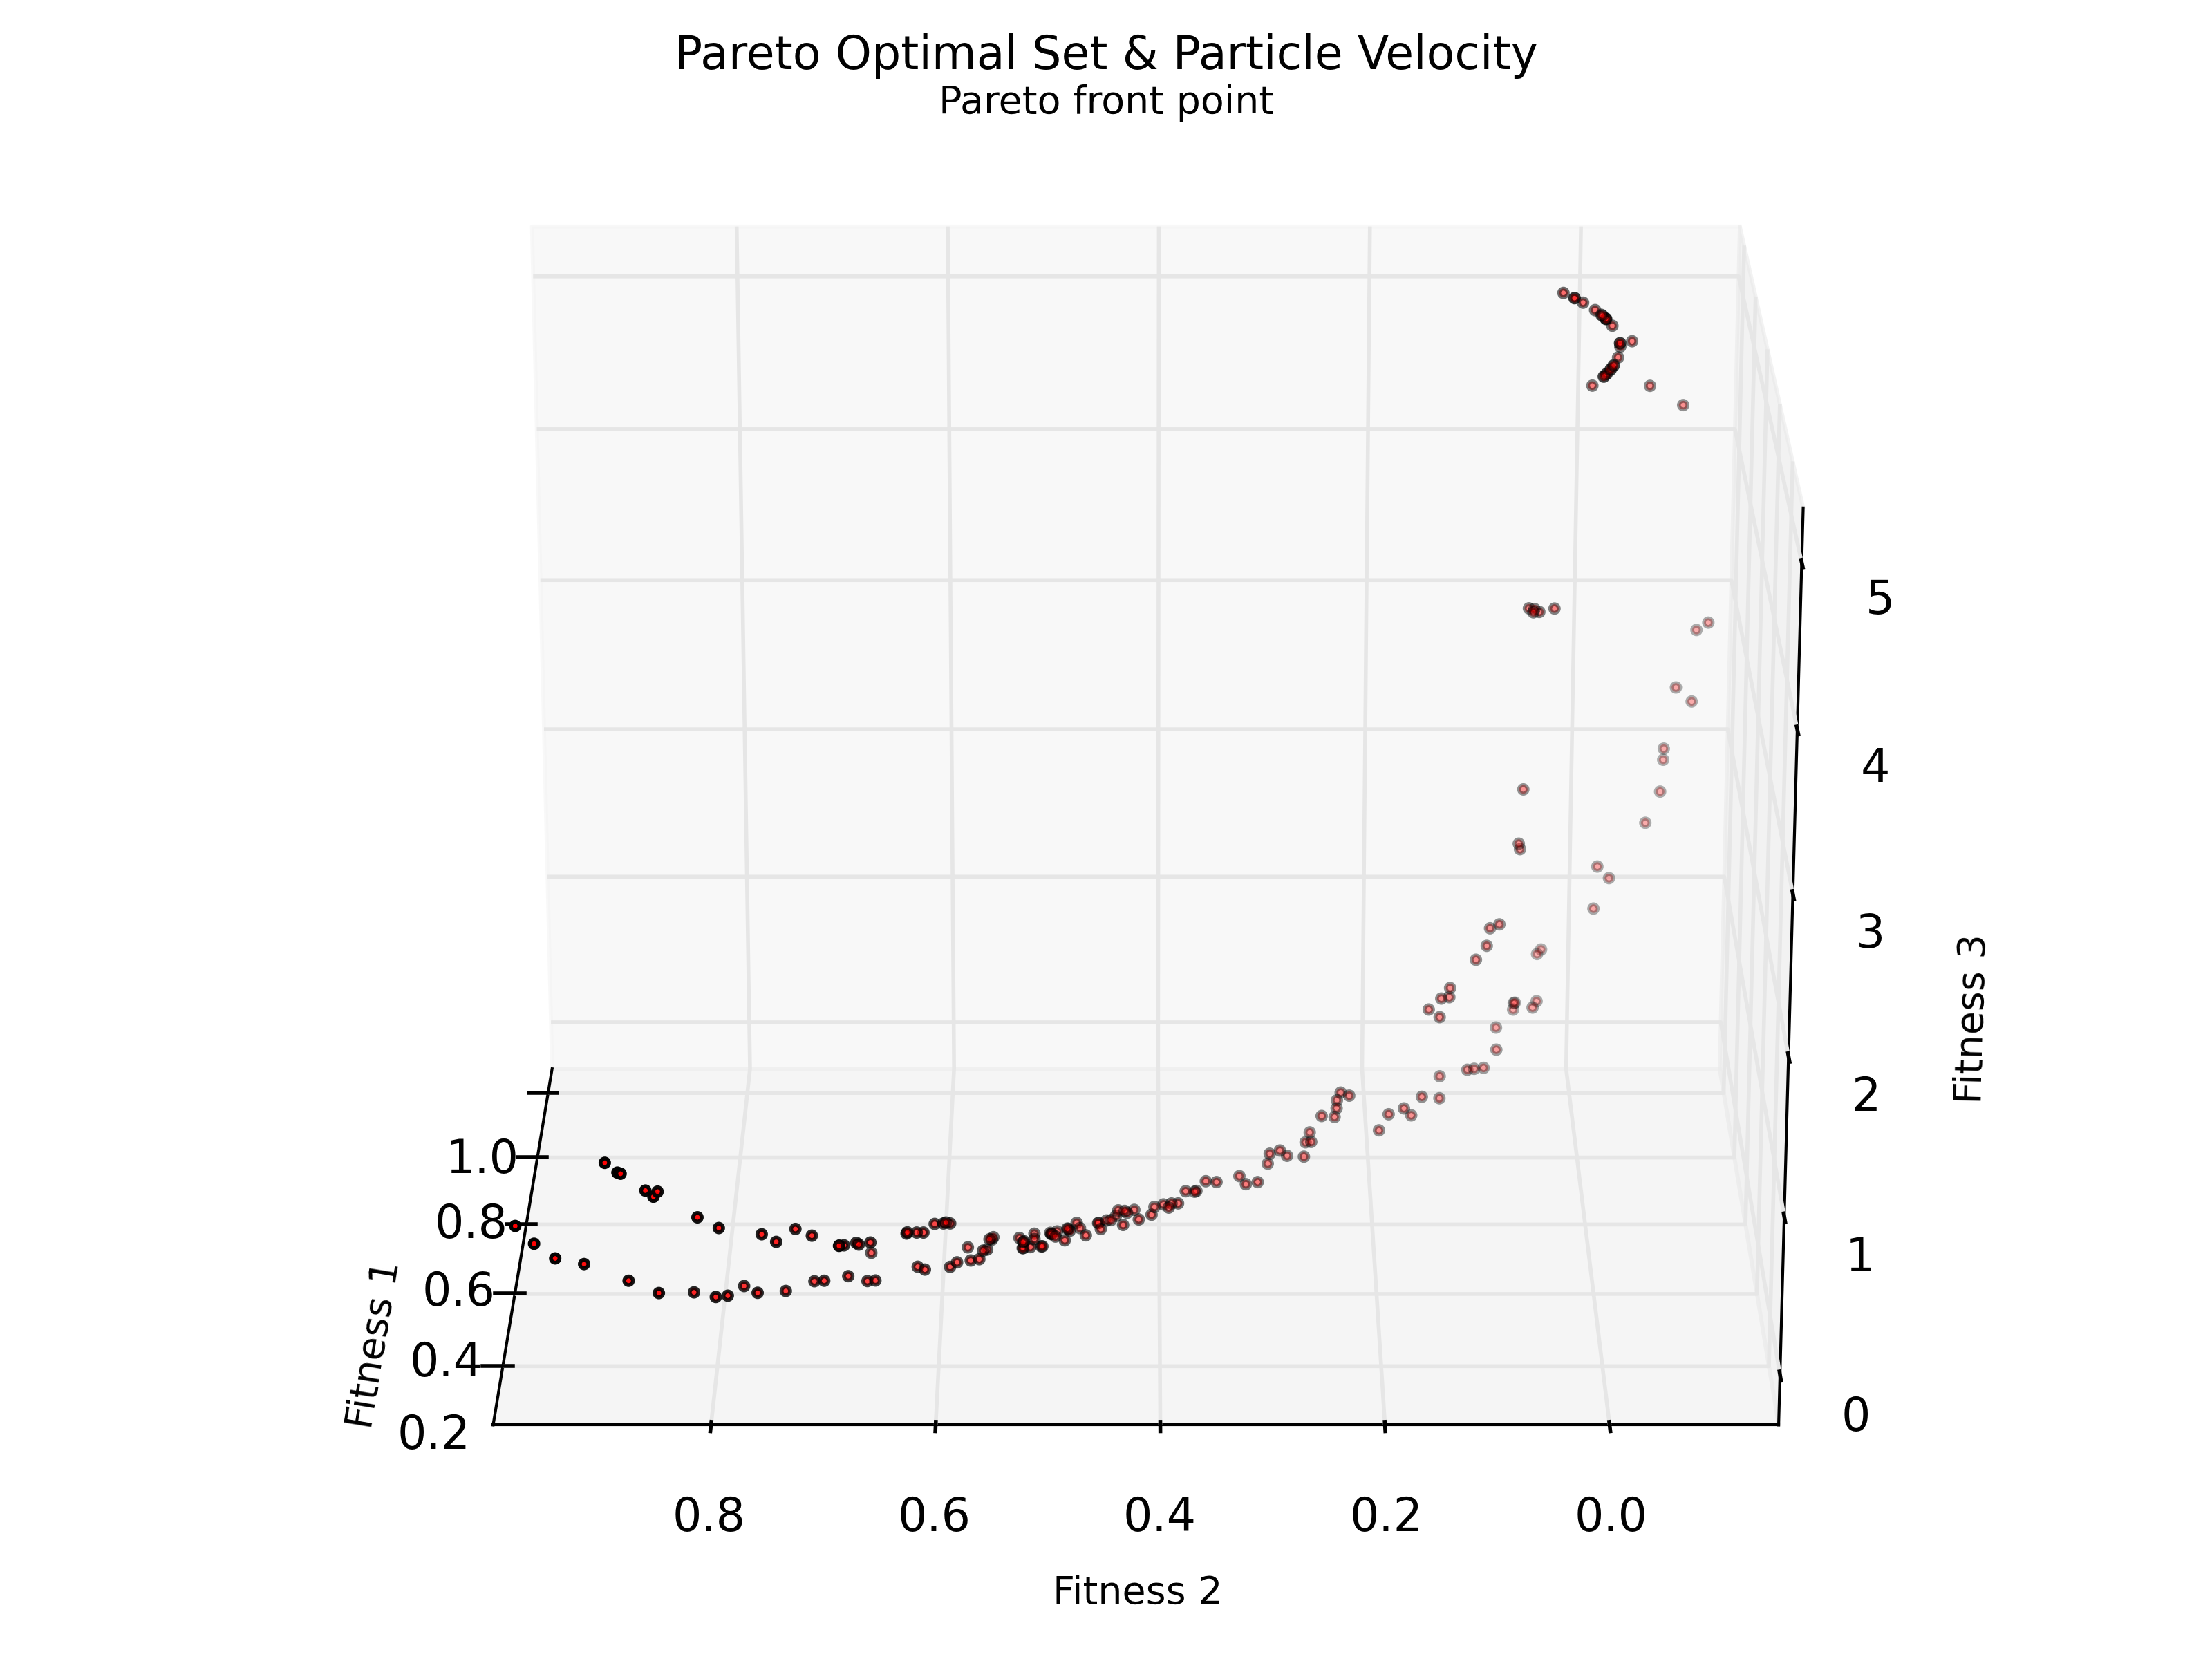
\includegraphics[width=0.8\textwidth]{./figs/3d.png}
        \caption{Plot of the run results image for three-objective artificial continious function.}\label{fig:3d}
\end{figure}

\begin{figure}
        \centering
    \centering
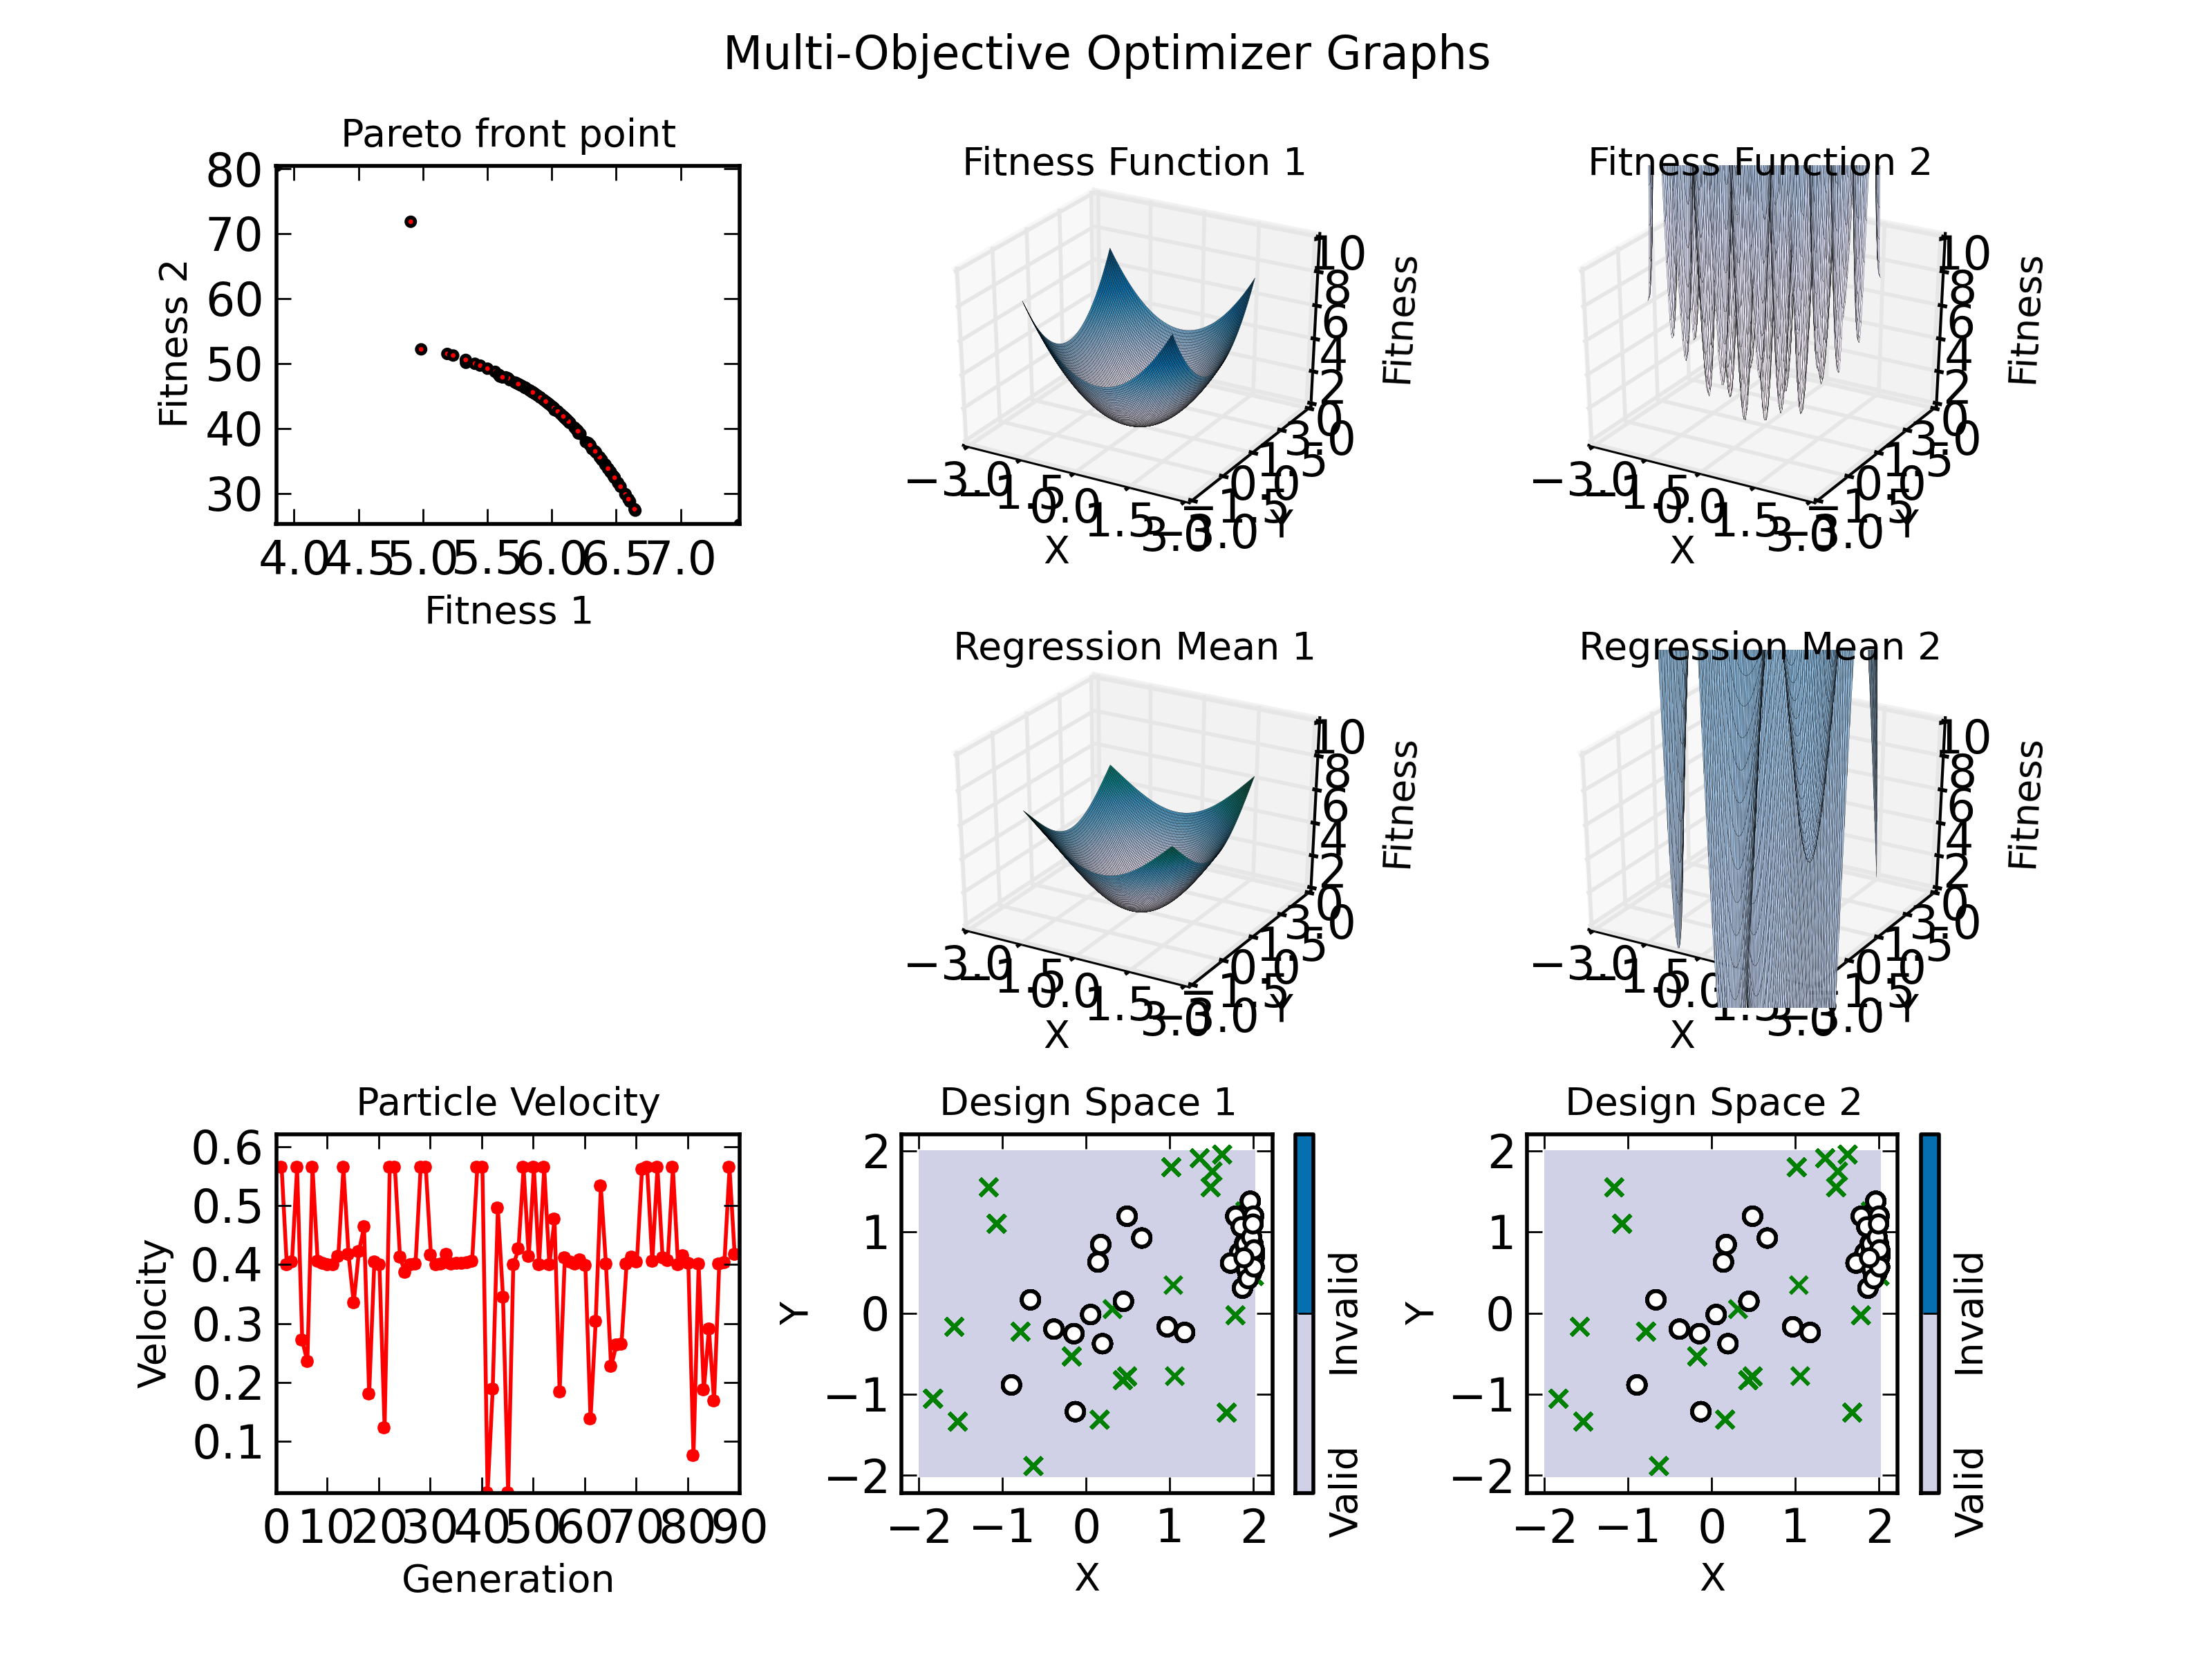
\includegraphics[width=0.8\textwidth]{./figs/max.png}
        \caption{Plot of the run results image for two maximization single-objective artificial continious functions.}\label{fig:max}
\end{figure}

\begin{figure}
        \centering
    \centering
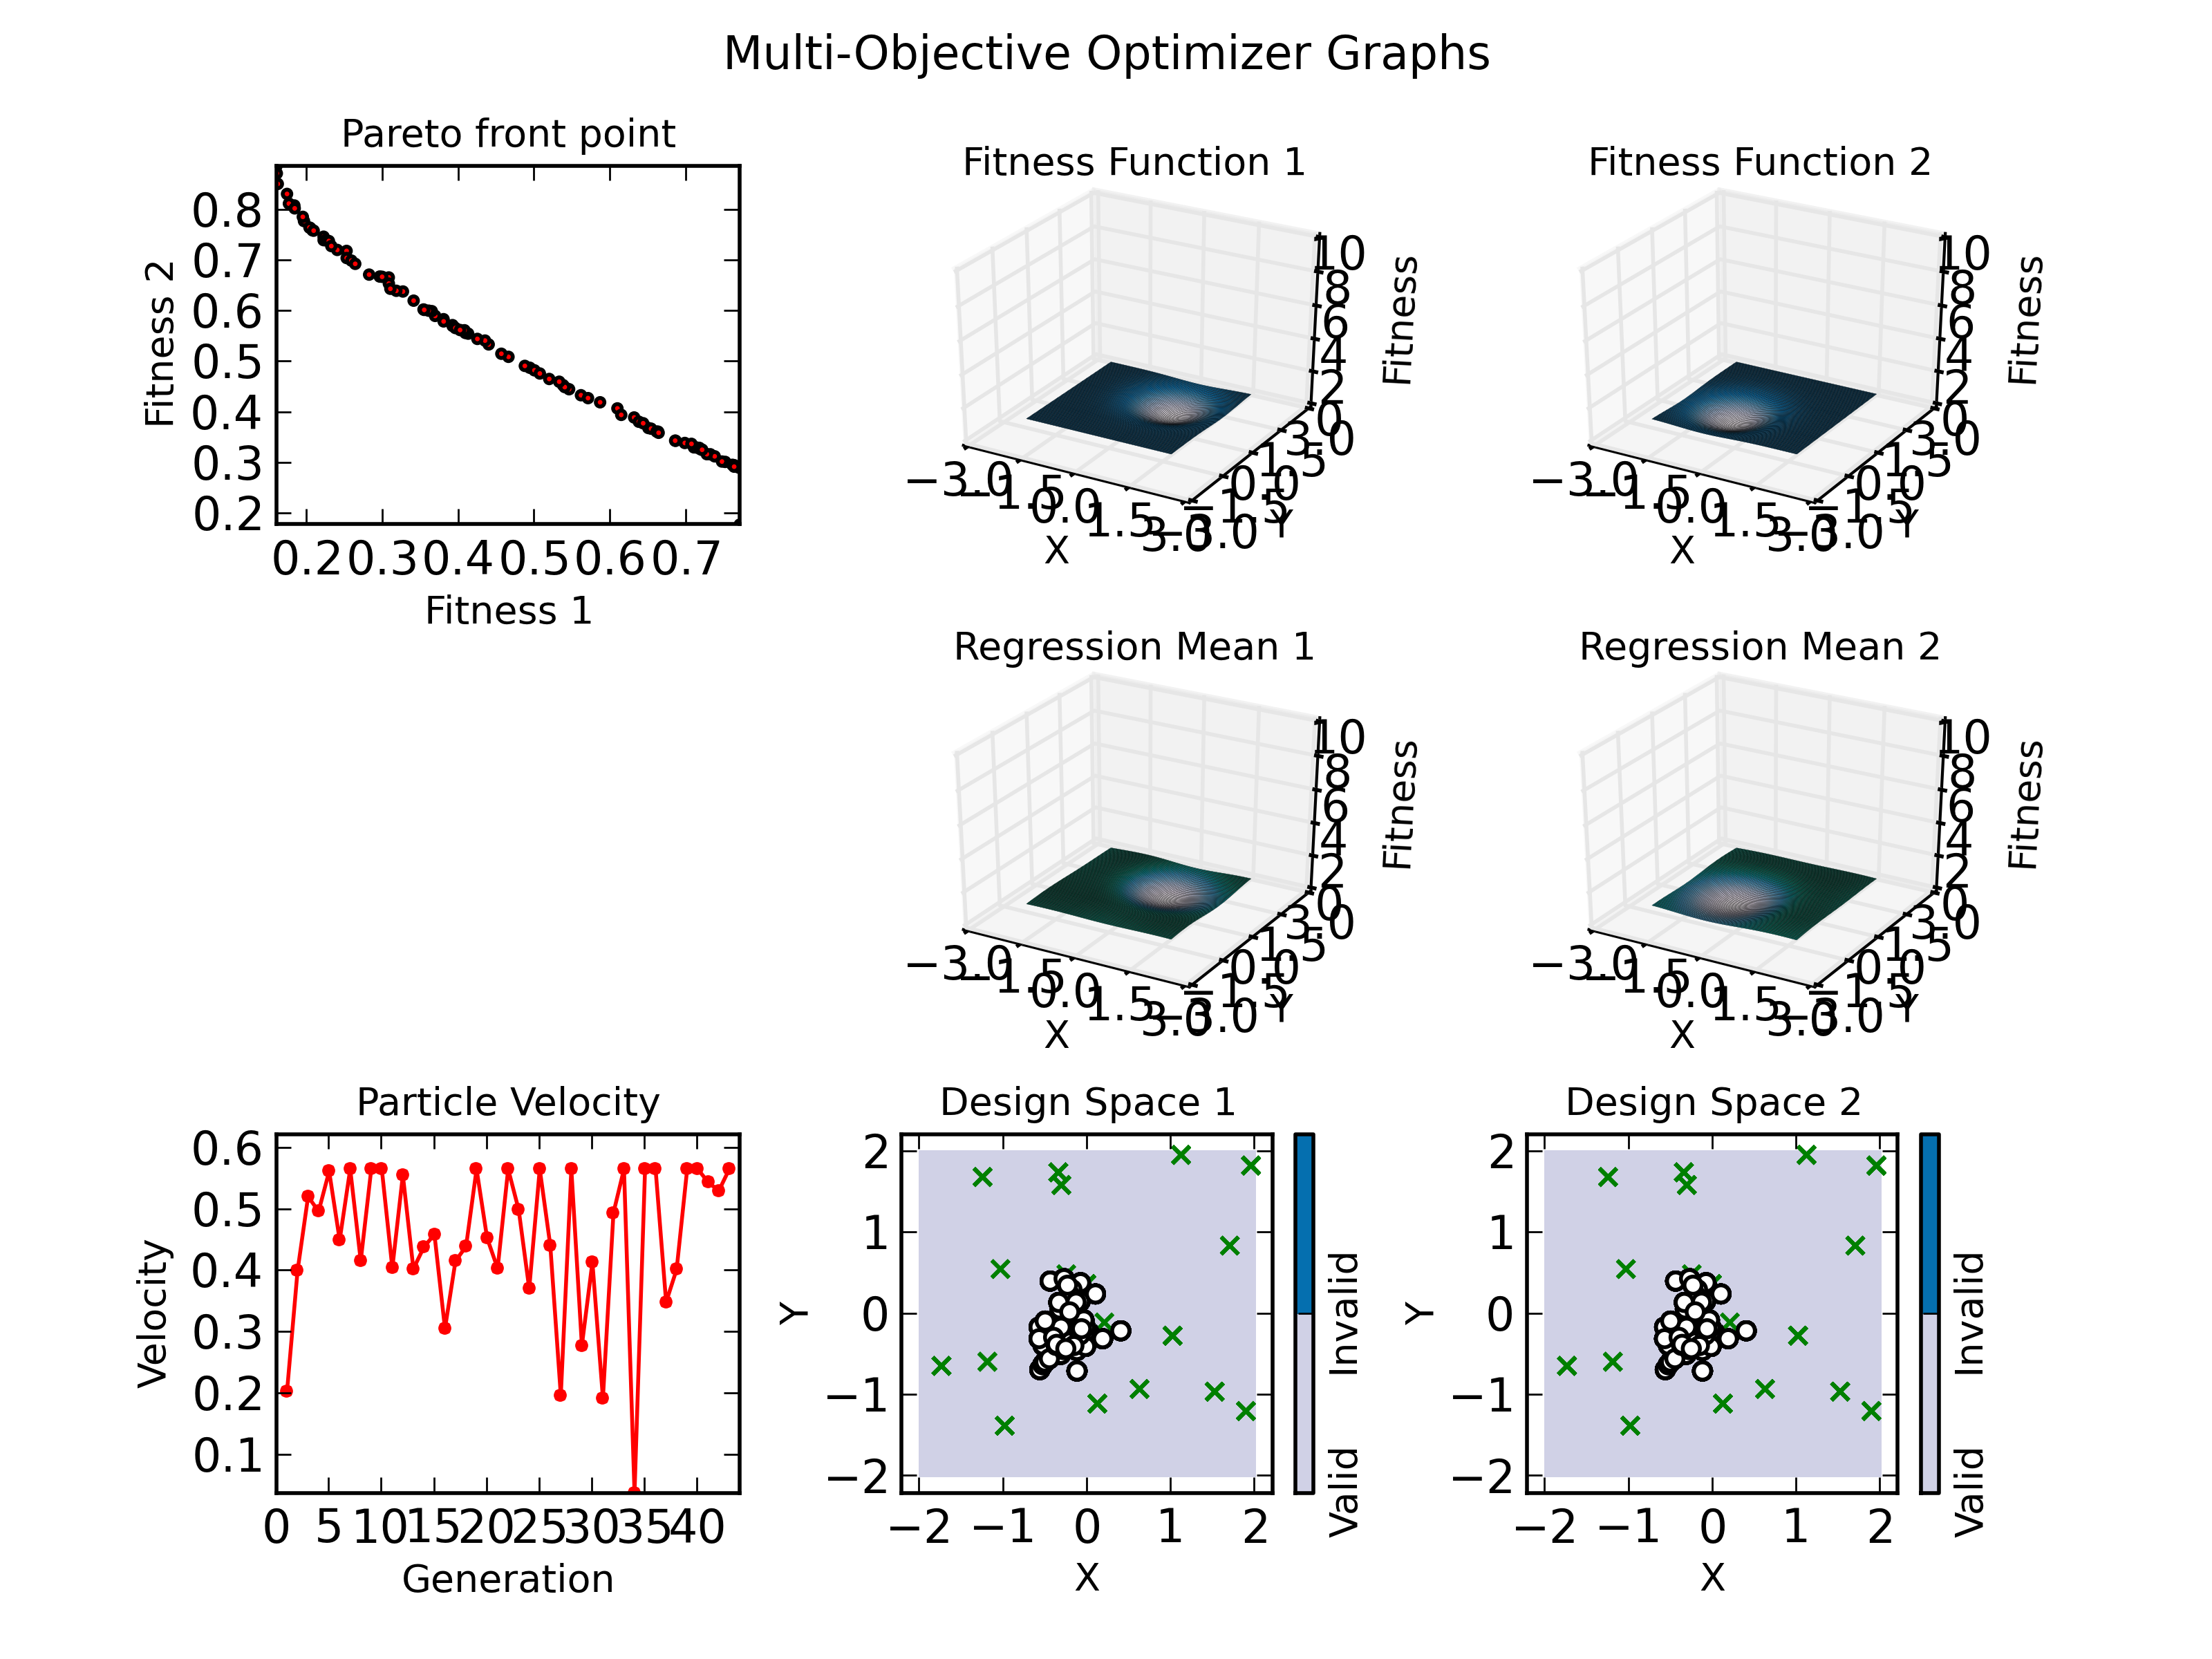
\includegraphics[width=0.8\textwidth]{./figs/fosna.png}
        \caption{Plot of the run results image for bi-objective artificial continious function.}\label{fig:fonseca}
\end{figure}

%\label{quadappbench}
As we can see in the first 3 images ( Fig.~\ref{fig:shron}, Fig.~\ref{fig:max} and Fig.~\ref{fig:fonseca}), which are all bi-objective optimization problem, the shape of the Pareto Optimal Set  $\mathcal{P}$ are all denote a reasonable approximation of the Pareto Front $\mathcal{PF}$. 

Notice that the plot of the design space shows the particles converge but not exactly in the same position, which is because the multi-objective optimization won't guarantee a best solution but a series of Non-dominated solutions. At last image ( Fig.~\ref{fig:3d}) for the 3D plotting of the 3-objective fitness functions, each axis represents a single fitness function and the results gives the  Pareto Optimal Set  $\mathcal{P}$ (now it is a surface instead of a line in bi-objective problems), which indicates the trade-off between these objectives.



\subsection{Comparison of approaches}
We compared the different approaches we used to design the \ac{mopso} by giving several runs of the trials on the same bi-objective fitness function: fonseca. For each approach we present a graph for the Pareto Front obtained from the trial (the most representative one) to indicate how good the approach is in approximating the Pareto Front (we expect it to be similar as Figure ). In addition, an average converge time (which obtained from over 10 trials each) has been presented for each approach to measure the converge property of them. Obviously, we prefer the one with less converge time and more accurate Pareto Front.

\subsubsection{Leader-retrieve methods}
We can see only slightly difference from the converging time ( Table.~\ref{tab:compare1})for all of the three solutions and the roulette method is slightly better than the others. The roulette selection method shows great performance on the shape of the Pareto Front ( see Fig.~\ref{fig:retrieve}), which is because its half-randomness property and also it avoids the aimless of a particle tracing the worse solution in least density solution.


\begin{figure}
        \centering
        \begin{subfigure}[b]{0.3\textwidth}
                \centering
                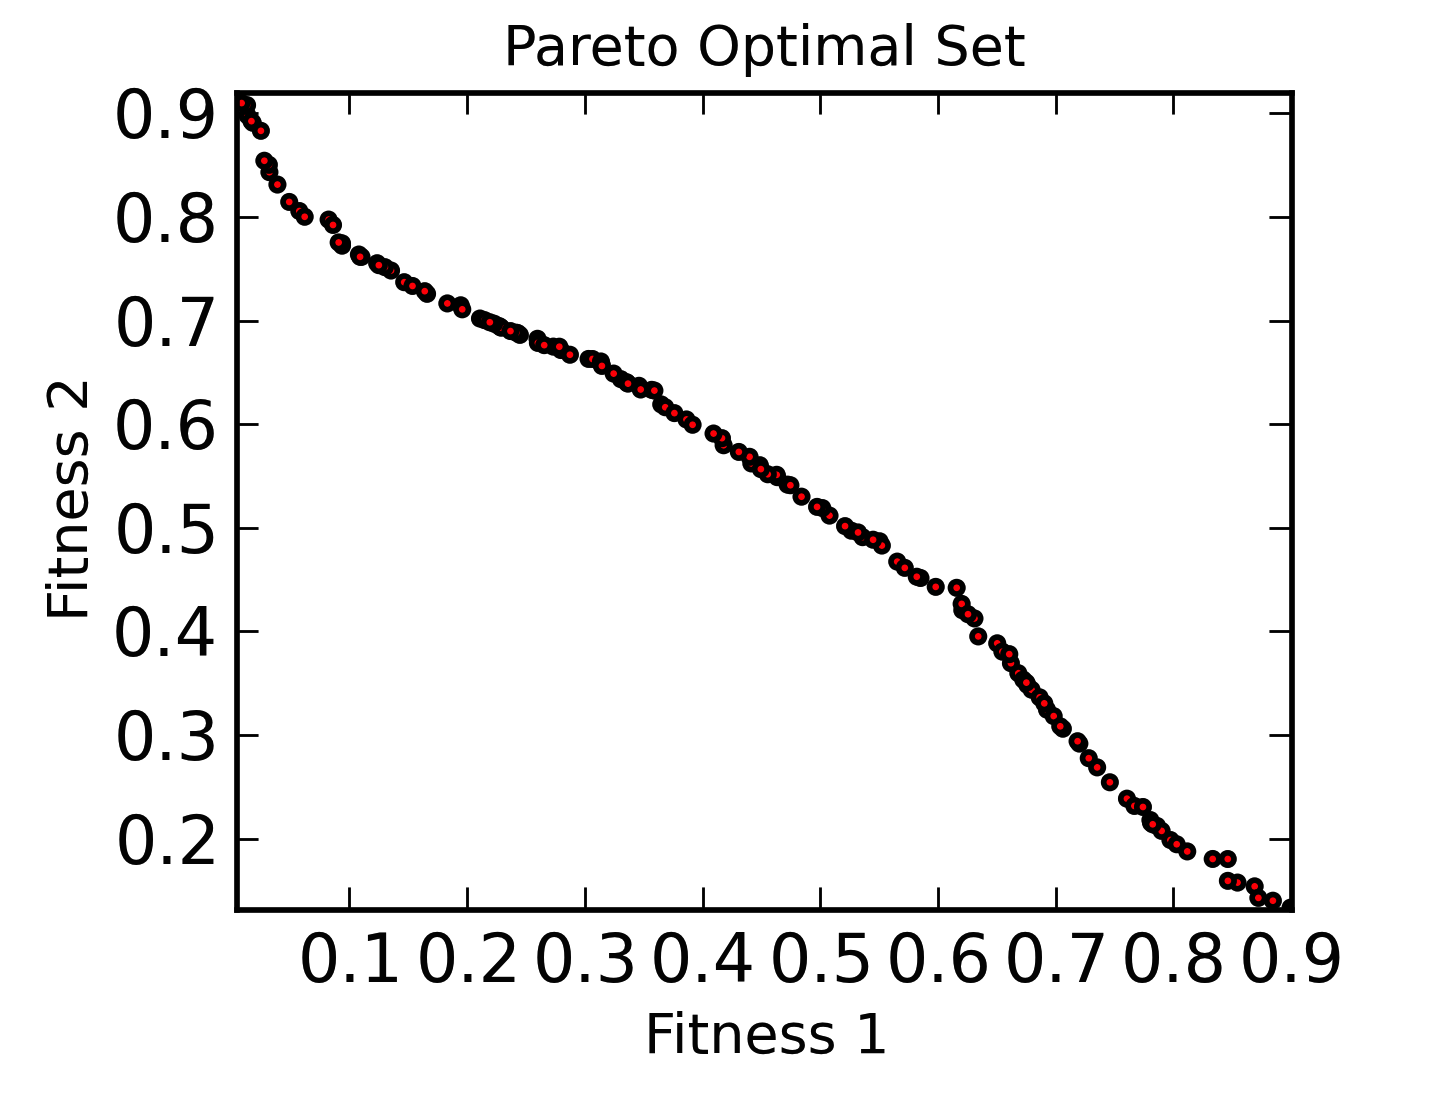
\includegraphics[width=\textwidth]{./figs/leastdensity.png}
                \subcaption{Least Density Method}
                \label{fig:ra}
        \end{subfigure}
        \begin{subfigure}[b]{0.3\textwidth}
                \centering
                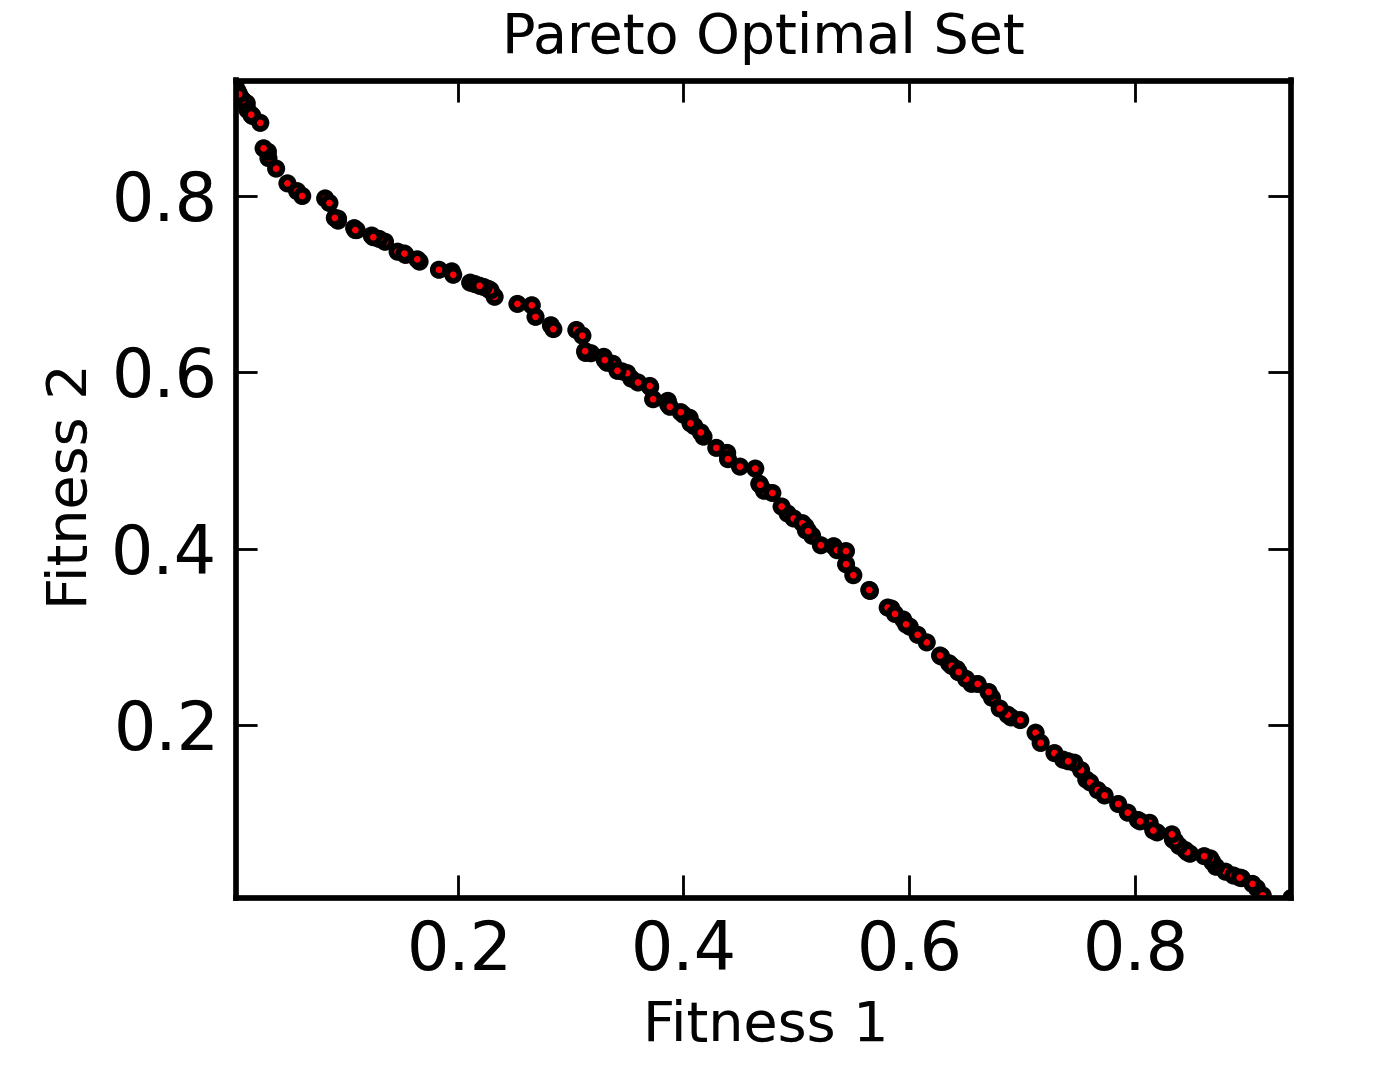
\includegraphics[width=\textwidth]{./figs/tournament.png}
                \subcaption{Tournament Method}
                \label{fig:rb}
        \end{subfigure}
        \begin{subfigure}[b]{0.3\textwidth}
                \centering
                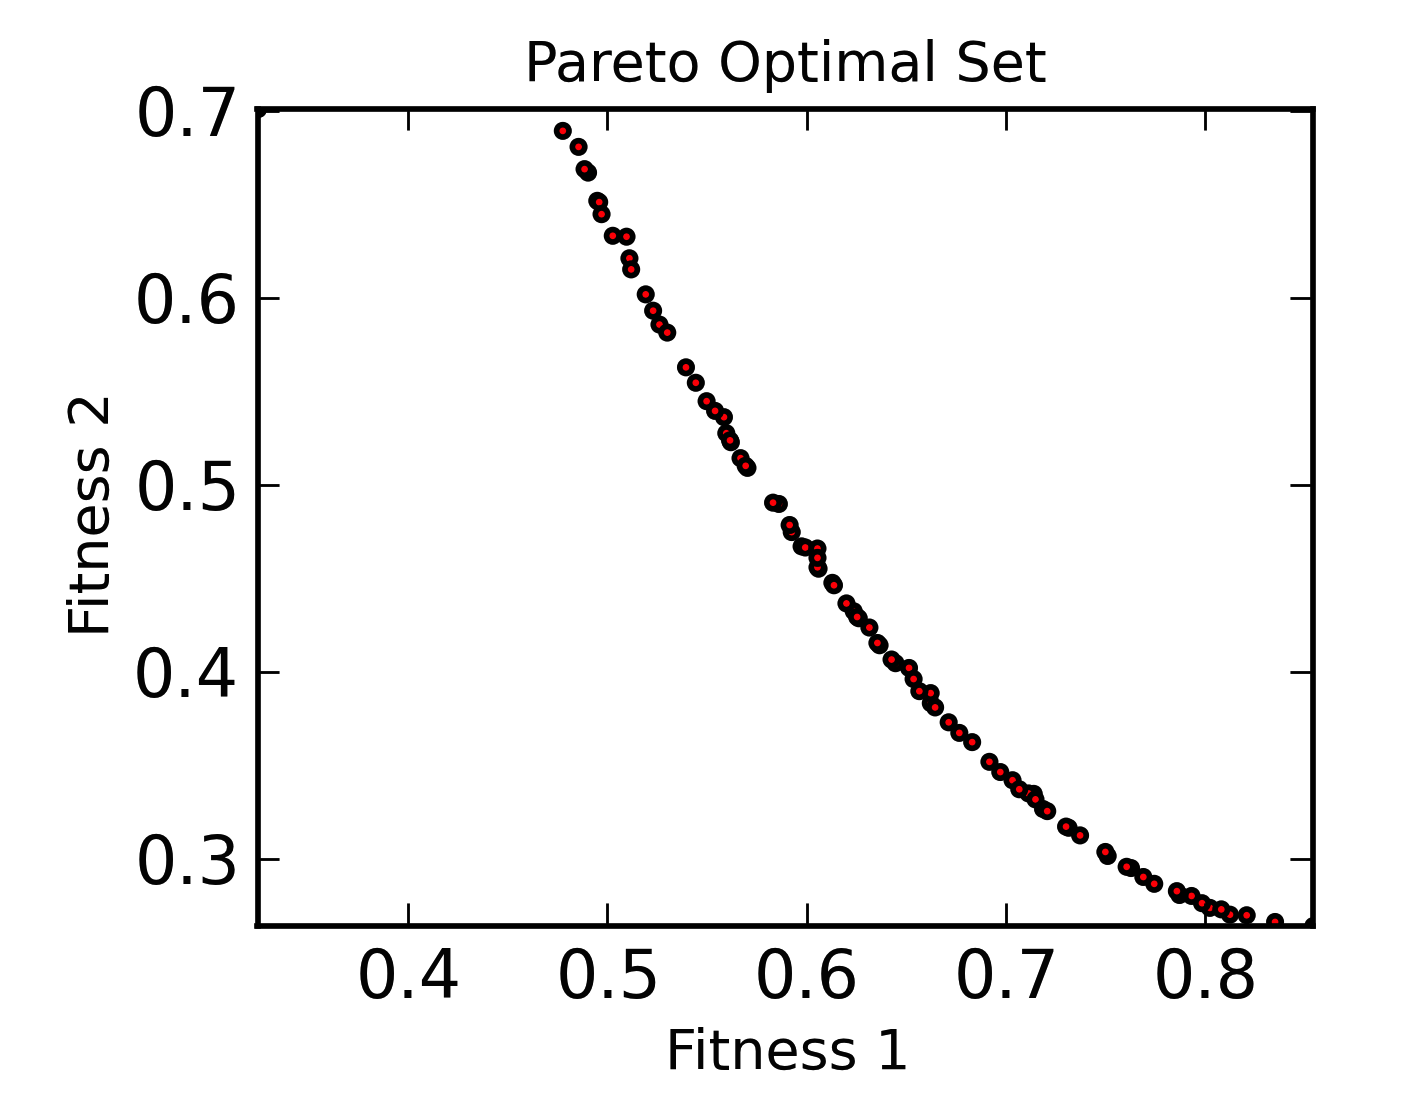
\includegraphics[width=\textwidth]{./figs/rolette.png}
                \subcaption{Roulette Method}
                \label{fig:rc}
        \end{subfigure}
        \caption{Plot of Pareto Optimal Set from three Leader-retrieve methods}\label{fig:retrieve}
\end{figure}

\begin{table}
  \caption{Average converge time for different Leader-retrieve of methods}  
  \label{tab:compare1}
    \begin{center}
\begin{tabular}{c|cccc} 
\toprule 
 %&  \multicolumn{3}{c}{$\epsilon_{rms}$ } \\
	$\mathbf{Methods}$   & $\mathbf{Average\ Converge\ Time (ms)}$\\
	\hline Least density particle &  1290 \\ 
         Tournament & 1360 \\
         Roulette selection & 1123\\
\bottomrule 
\end{tabular} 
\end{center}
\end{table}

\subsubsection{Non-dominated Retain methods}
For the retain methods,  the $\epsilon$-dominate method is obviously better concerning both measurements as presented in the Table.~\ref{tab:compare2}  and the Fig.~\ref{fig:retain}: the average converging time is two-thirds of the simple retain methods and the Pareto front of $\epsilon$-dominate method shows a much better shape than another.
\begin{figure}
        \centering
        \begin{subfigure}[b]{0.4\textwidth}
                \centering
                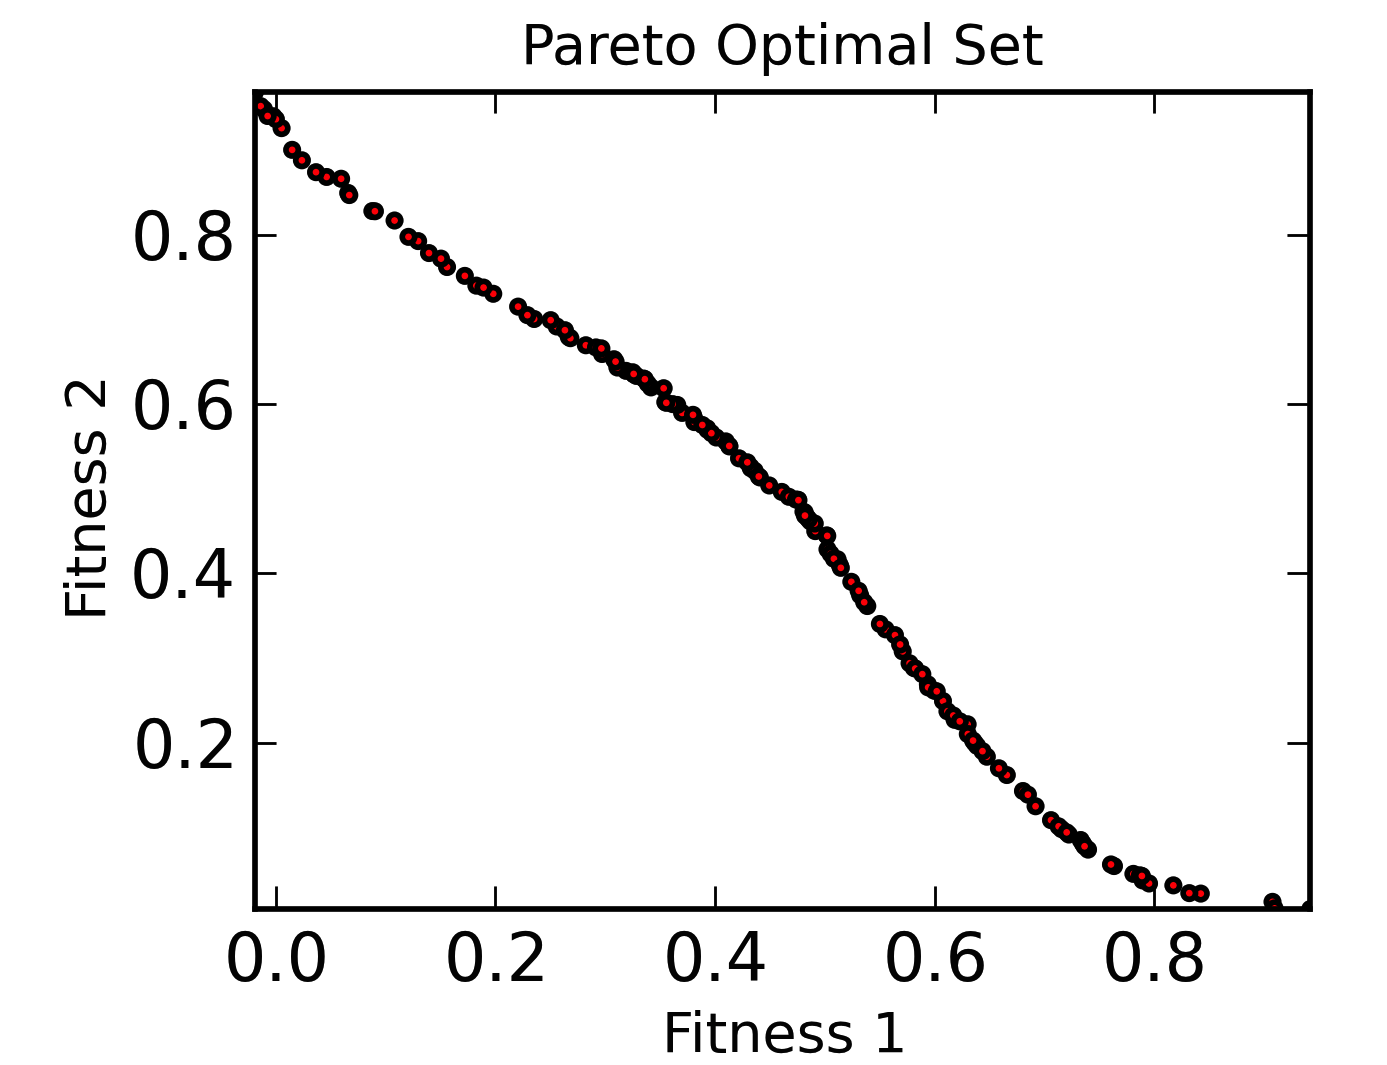
\includegraphics[width=\textwidth]{./figs/simpleretain.png}
                \subcaption{Simple Retain Method}
        \end{subfigure}
        \begin{subfigure}[b]{0.4\textwidth}
                \centering
                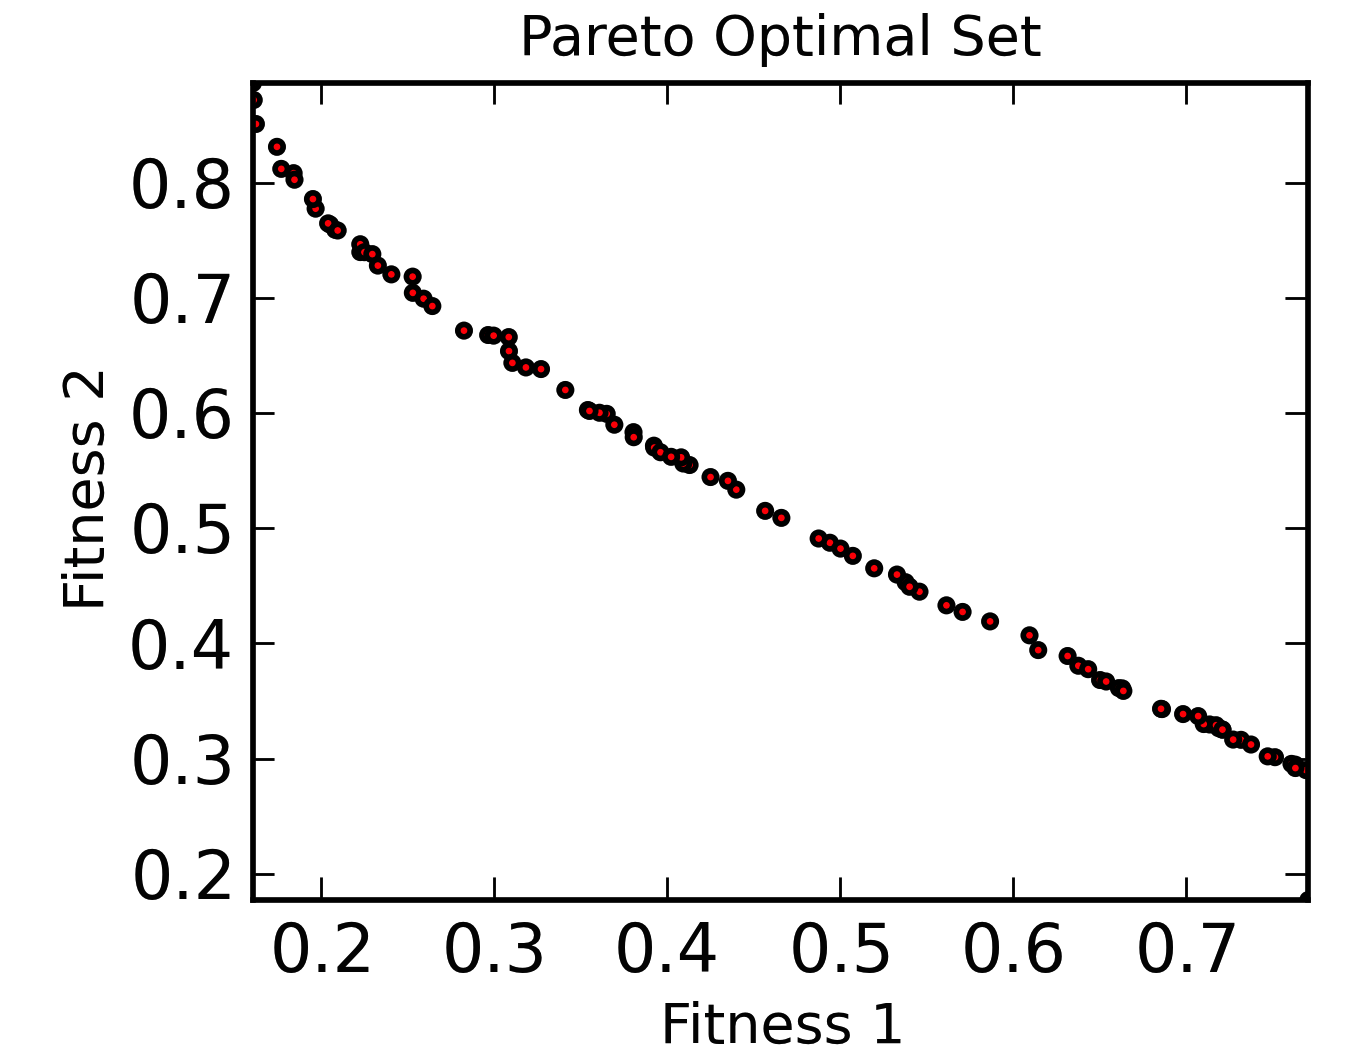
\includegraphics[width=\textwidth]{./figs/edominance.png}
                \subcaption{$\epsilon$-dominate Method}
        \end{subfigure}
        \caption{Plot of Pareto Optimal Set from two Non-dominated Retain methods.}\label{fig:retain}
\end{figure}

\begin{table}
  \caption {Average converge time for different Non-dominated Retain of methods}  
  \label{tab:compare2}
    \begin{center}
\begin{tabular}{c|cccc} 
\toprule 
 %&  \multicolumn{3}{c}{$\epsilon_{rms}$ } \\
	$\mathbf{Methods}$   & $\mathbf{Average\ Converge\ Time (ms)}$\\
	\hline Simple Retain with replacement: &  1330 \\ 
         $\epsilon$-dominate retain & 890 \\
\bottomrule 
\end{tabular} 
\end{center}
\end{table}


\subsubsection{Neighbor Density Estimators}
At last, as we can see in the Table.~\ref{tab:compare3} and Fig.~\ref{fig:density}, the two methods produce almost the same results on both the converge time and Pareto front approximation, so we declaim that both of them are suitable for this application and we will choose one randomly.


\begin{figure}
        \centering
        \begin{subfigure}[b]{0.4\textwidth}
                \centering
                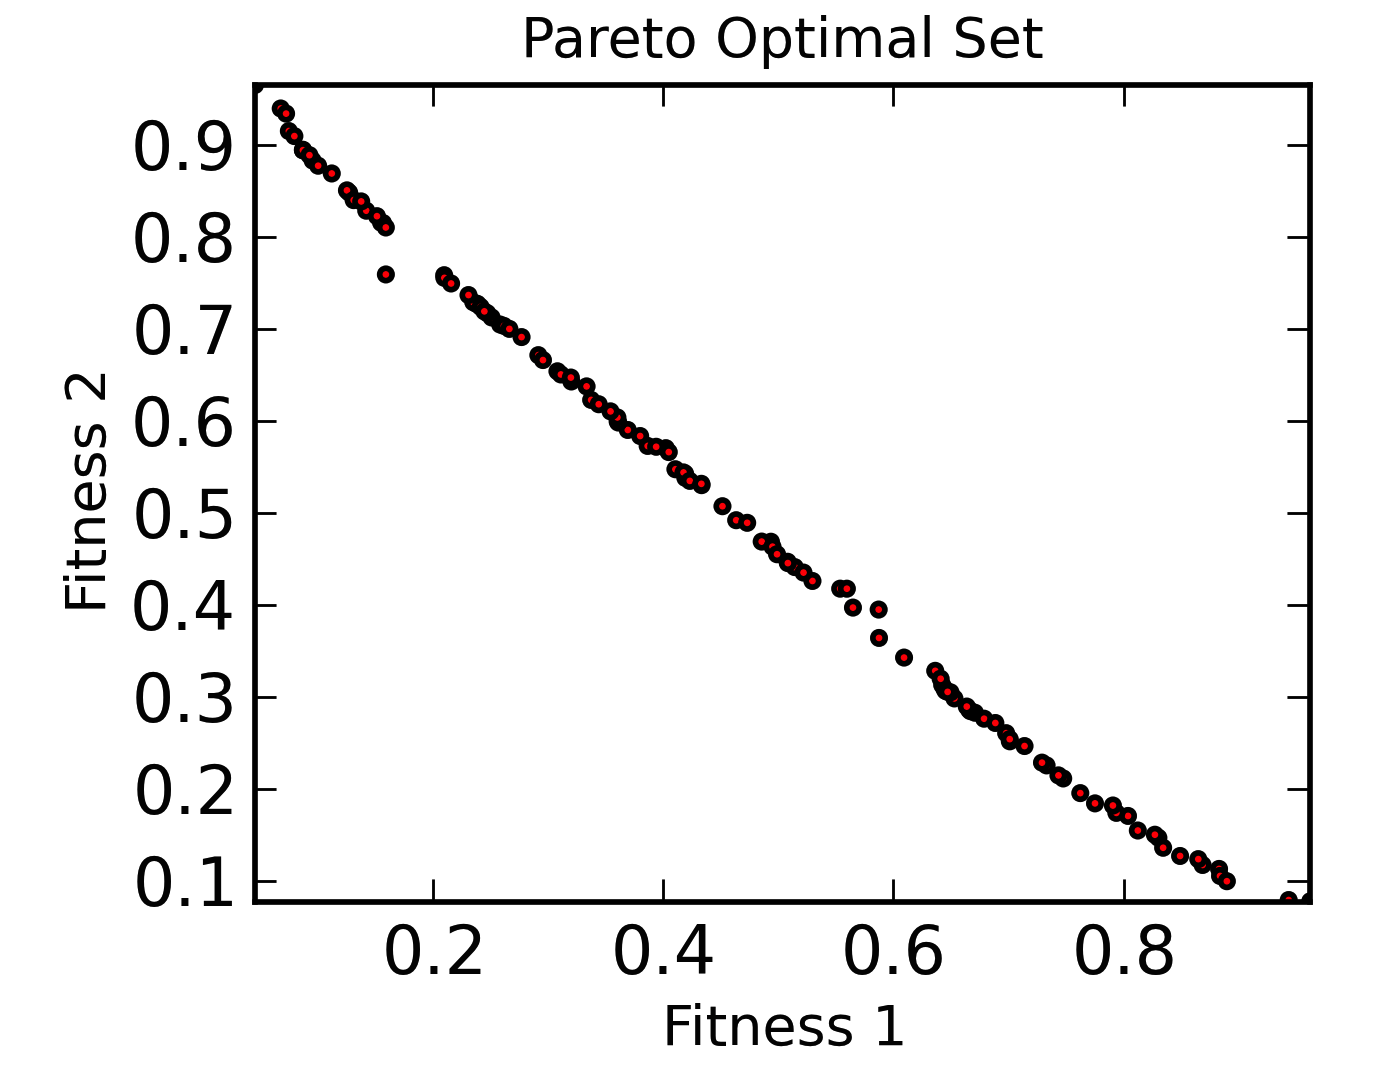
\includegraphics[width=\textwidth]{./figs/nearst2.png}
                \subcaption{Nearest-$2$ neighbors}
        \end{subfigure}
        \begin{subfigure}[b]{0.4\textwidth}
                \centering
                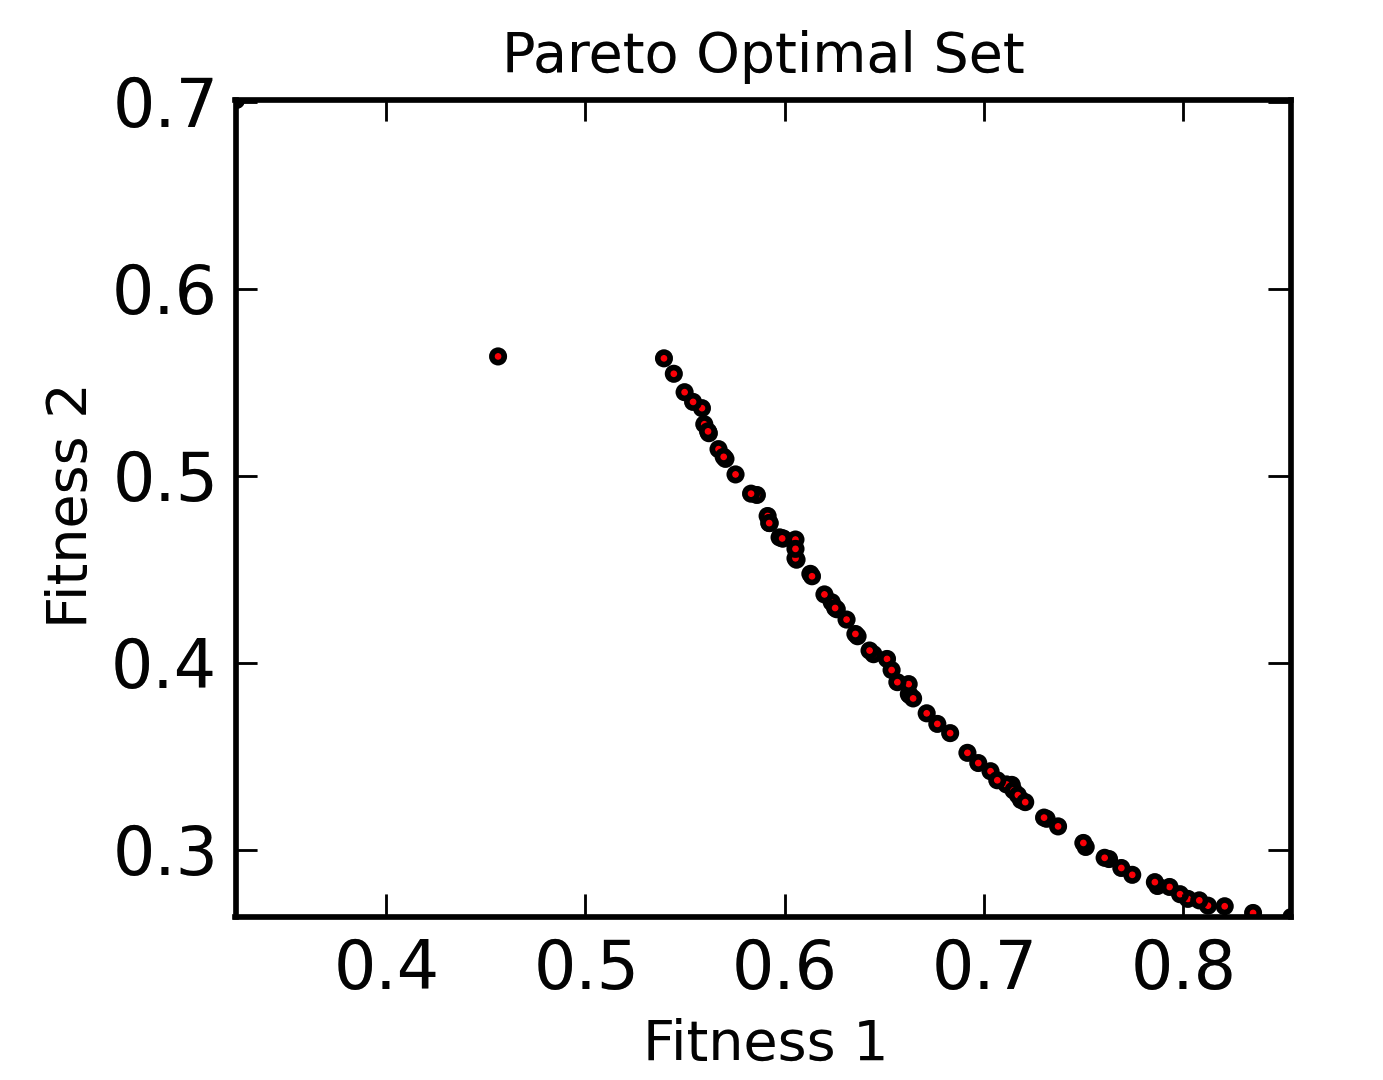
\includegraphics[width=\textwidth]{./figs/niche.png}
                \subcaption{Niche neighbors}
        \end{subfigure}
        \caption{Plot of Pareto Optimal Set from two Non-dominated Retain methods.}\label{fig:density}
\end{figure}
\begin{table}
\caption {Average converge time for different Neighbor Density methods}\label{tab:compare3}
 \begin{center}
\begin{tabular}{c|cccc} 
\toprule 
 %&  \multicolumn{3}{c}{$\epsilon_{rms}$ } \\
	$\mathbf{Methods}$   & $\mathbf{Average\ Converge\ Time (ms)}$\\
	\hline Nearest-$2$ neighbors &  1232 \\ 
         Niche neighbors & 1295 \\
\bottomrule 
\end{tabular} 
\end{center}
\end{table}


From these results, we can now claim that the (roulette or tournament) + $\epsilon$-dominate  + (Nearest-$k$ neighbors or Niche neighbors) are the best combinations for the current application. 
Through all of the results, we can now decline that our design is correct and can efficiently solve the Multi-Objective Machine Learning Optimization problems on artificial continuous fitness functions. There are a little bit more work to do in the future to extend the current evaluation to discrete fitness functions which is actually the optimazation of the FPGA architecture want to achieve. The result is predictable to be good because in our previously work is successful on real FPGA problem such as Reconfigurable Software-defined Radio and Quadrature Method-based Application \cite{arc2012MLO}. The further evaluation on the FPGA will be carried through the following steps:
\begin{enumerate}\addtolength{\itemsep}{-0.1\baselineskip}  
\item For each objectives, construct a fitness function which receive parameters produces a single fitness value.
\item When apply the update of the particle's position, the new position must be dithered to a discrete parameter space.
\item Then run the system to get a Pareto Optimal Set of the parameter space.
\item Choose a best one or a best subset artificially within the Pareto Optimal Set.
\end{enumerate}


By doing all of these, we can get an Pareto Optimal Set concerning several FPGA objectives, i.e. Speed, Accuracy, Power/Energy consumption, which can make a trade-off between different objectives. It is noticeable that this method successfully employs a completely new way of exploring the FPGA architecture within multi-objective scope and the result gain from it is unlikely to be achieved by a human FPGA designer within a small amount of time to consider an array of fitness functions and make best of them.

\section{Regression Test}
\subsection{Regression Test Design}
Regression testing is an integral part of the extreme programming software development method. In this method, design documents are replaced by extensive, repeatable, and automated testing of the entire software package throughout each stage of the software development cycle \cite{regression}. In the corporate world, regression testing has traditionally been performed by a software quality assurance team after the development team has completed work.
Regression testing can be used not only for testing the correctness of a program, but often also for tracking the quality of its output. In our project, the regression test is very important since the quality on how good a MLO is partly on how long it takes to achieve the termination condition and how many generations it takes for the whole trial. One possible way to achieve this goal is to keep a golden result file in the same folder of configuration script and every time we run a trial based on this configuration file, it will be read and used to compare with the current result to see how good the current result is. Thus a golden file is created once and to be compared later with latter design. In every run of the trial, two main fields of criterion are measured:
\subsubsection{counters}
\begin{list}{$\bullet$}{\itemsep 0.5ex}
\item Counter "g": Used for measuring how many generations in this run of MLO, obviously we want to find optimal solution to reduce the generations to reach the termination condition.
\item Counter "it": Used for measuring how many times the trial evaluate the fitness funtions. Again this should be as less as possible because each evaluation of the fitness will occupy the computing capacity of the host machine it runs. 

\end{list}

\subsubsection{timers}
\begin{list}{$\bullet$}{\itemsep 0.5ex}
\item Model Training Time: The model predict time is the time for the regressors to train the surrogate model. As this is the most time-consuming part in the whole program, it becomes the bottleneck for the improvement of the design. A substantial effort has been done to improve this part, so the time can be used as how good the current training parameters (including the kernel function, training algorithm, etc.).
\item Model Predicting Time: The prediction time for the models also consume some time but not so much currently which is negligible but we still need to measure it for the future use.
\item Running Time: The running time for the whole program is a important one since it tell us how long it takes to run this trial runs including the training, predicting and the meta-heuristic run time, this is a primary comparing method for measuring the trials. However, this is not always the case because two different trial with the same configuration and fitness function may have huge difference on the running time since the meta-heuristic is non-determinate. In that case, a good method to eliminate this is to have several trials running consecutively and then take the average of the running time.
\end{list}

\subsection{Implementation}
As discussed above, to develop a scheme for discovering how good current solution is when compared to the golden solution is very important. There are mainly three parts within this implementation:
\begin{list}{$\bullet$}{\itemsep 0.5ex}
\item The maintain of the trial information: In the implementation a 'snapshot' function is used for take a virtual 'snapshot' for the trial, which contains all the information (name, budget, timers, counters, etc) for the trial. For the other class to get the trial information, one call to this snapshot is enough when the trial finishes and then passed to the processing function for the further comparison.
\begin{figure}
        \centering
    \centering
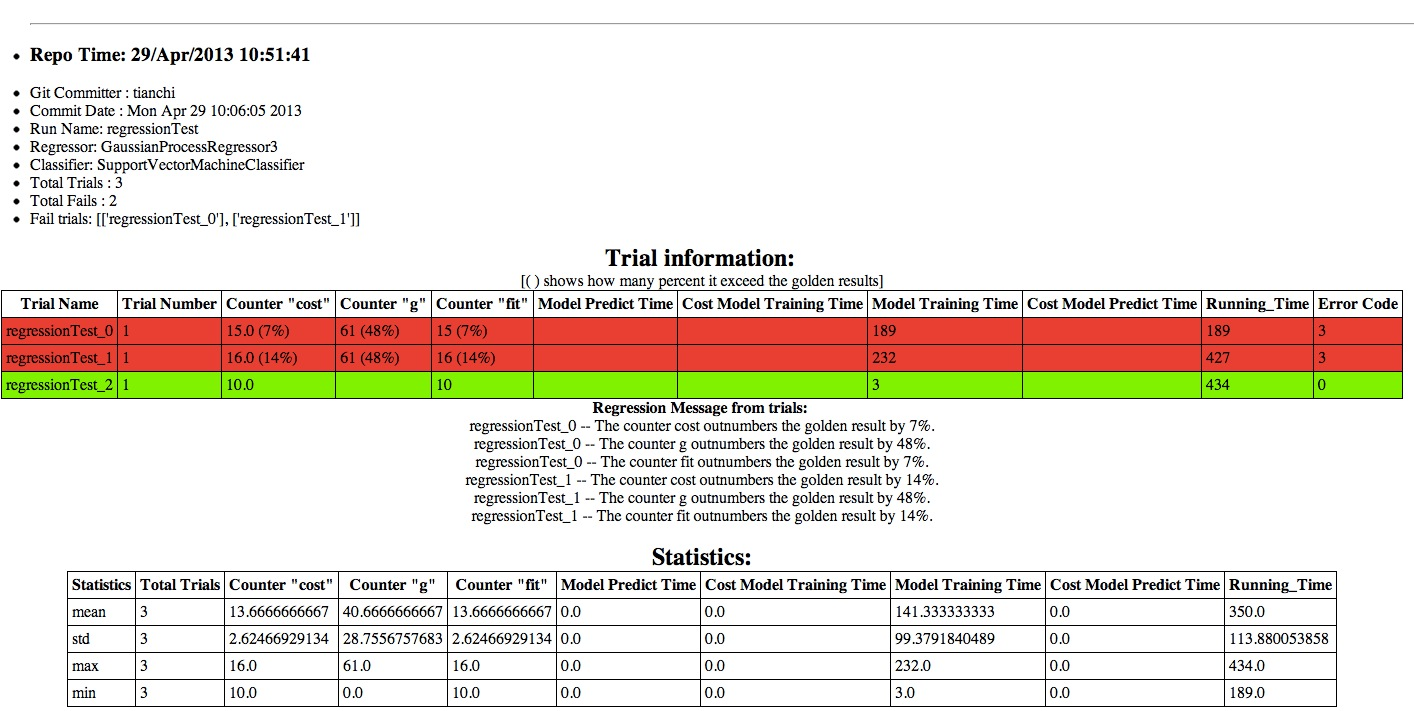
\includegraphics[width=1\textwidth]{./figs/regTest.png}
        \caption{An example of Regression Test Html Report}\label{fig:regtest}
\end{figure}

\item The comparison of the current solution with the golden result: For every measurement of the trial, the comparison with the golden result is done and the outnumber percentage over the golden result is calculated which will give a more straightforward way for further comparing between any two new trials. Furthermore, the generation information and the fitness counter are compared with the budget, which will used as a mark for the trial fails or not. In addition, the statistic information is calculated across all the trials in a single run, which contains the mean, standard deviation, max value and min value of all the attributes calculated above. 
\item The design and implementation of the details of the report and techniques to achieve this: We choose to use two different packages in python (HTML and pisa) to create the html file and the pdf report respectively. It is important to keep the trial information like the github version and the run configuration in the report, which is easy to implemented as list using the html package. The content in the head of the report is designed as follows:
\begin{list}{$\bullet$}{\itemsep 0.2ex}
\item Repo Time: 17/Apr/2013 20:49:52
\item Git Committer : tianchi
\item Commit Date : Fri Apr 12 17:23:37 2013
\item Run Name: example
\item Regressor: GaussianProcessRegressor3
\item Classifier: SupportVectorMachineClassifier
\item Total Trials : 1
\item Total Fails : 1
\item Fail trials: 'example\_0'
\end{list}
\end{list}
The next part in the report comes with the trial information on the counters and timers, and there are messages pop out for this trial under the table. It is worth to be mentioned that when the trial fails, the corresponding row will be marked red compared with the successful one in green. As discussed above, the statistics measure is very important to eliminate the randomization of the meta-heuristic so it is displayed under the trial information. The Fig.~\ref{fig:regtest} is an example of the html report.



\section{Conclusions and Future Work}
Based on the previous successful work on the MLO, we present a new method on the Multi-objective Machine Learning Optimizer on the FPGA architecture design. The Multi-Objective MLO which mainly based on Pareto optimal solution can offer superior performance on the exploration on the parameter space in respect to several objectives and yielding "trade-off" between these objectives, which may including performance measure like power consumption and accuracy. Several approaches to achieve best performance of the approximation of the Pareto Front are done and the evaluation and comparison are shown, which indicate the good performance of using a density estimator and the $\epsilon$-Dominance to manage the Pareto Optimal Set. Furthermore, the multi-objective optimization approach that we have presented is only tested on artificial examples, with additional work, may be simply extended to a multitude of FPGA applications which offer a discrete fitness functions.

Future works for the Multi-Objective MLO is mainly about the improvement of the performance: apply more density measures and adjust the parameters used in the algorithm to be fast to converge; extend the currently artificial continuous test function to discrete optimization problem on the real FPGA applications; improve the modeling algorithm to reduce modeling error and time because now modeling is the main bottleneck which consume a majority of time running on the application. 

\section{What I learned}

\subsection{FPGA}
FPGA is not a familiar technique for me the only thing I know before is a single application often has multiple computationally intensive kernels that can benefit from acceleration using custom or reconfigurable hardware platforms, which is usually called field-programmable gate arrays (FPGAs). Then for the reconfigurable applications whose behavior can be modified by changing a few input parameters before execution are usually optimized manually, which on the contrary can be done by the optimizer automatically and this is completely a new area and it arouse my strong interest to research more on it.

\subsection{Maxeler Platform for Acceleration of Dataflow programming}
During the project I took part in the dataflow computing course operated by Maxeler Technology, which is extremely useful for me to apply my current Multi-Objective algorithm in the real FPGA applications. The dataflow computing was popularized by a number of researchers in the 1980's, in which an application is considered as a dataflow graph of the executable actions; as soon as the operands for the action are valid, the action is executed and the result is forward to the next action in the graph. In a Dataflow application, the program source is transformed into a Dataflow engine configuration file, which describes the operations, layout and connections of a Dataflow engine. Data can be streamed from memory into the chip where operations are performed and data is forwarded directly from one computational unit ("dataflow core") to another, as the results are needed, without being written to the off-chip memory until the chain of processing is complete.There are three applications I was doing for exercise and they are written in Java: 
\begin{list}{$\bullet$}{\itemsep 0.5ex}
\item Graph brightness adjustment: use the dataflow engine (DFE) to adding value to each pixel; 
\item Gamma Correction: use DFE to transfer the linear input image to the output image; 
\item Stream Offsets: read data from different locations with a stream. An example of the dataflow programing is shown in Fig.~\ref{fig:dfe}
\end{list}
 \begin{figure*}
     \centering
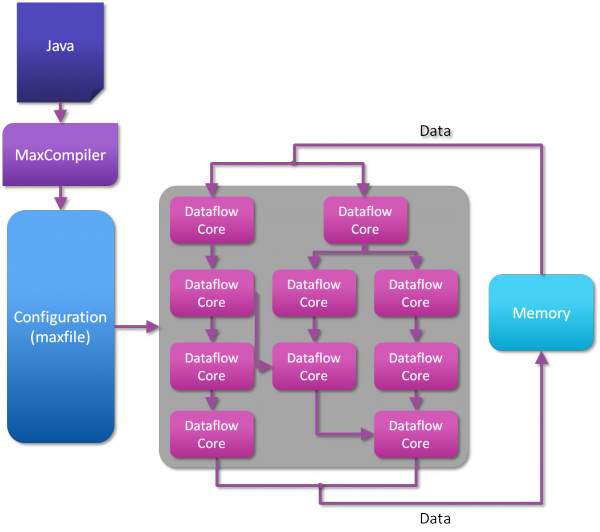
\includegraphics[width=0.6\textwidth]{./figs/DFE.png}
        \caption{Computing with dataflow cores}     
           \label{fig:dfe}
  \end{figure*} 

\subsection{Machine Learning Optimizer}
As discussed above reconfigurable applications whose behavior can be modified by changing a few input parameters before execution are usually optimized manually. This is a very tedious task, as the designer has to analyze the application, create benchmarks (fitness functions) and run the application with different combinations of input parameters .The objective of the MLO algorithm is to minimize the number of fitness function evaluations when solving a parameter optimization problem, which is clearly more beneficial than traditional approaches, when the fitness function takes a long time to return. The motivation for this was for optimizing parameters when designing heterogeneous computer systems, but it is useful in any parameter optimization problem with a time-consuming fitness function.

\subsection{Meta-heuristic}
The PSO and Multi-Objective PSO are the main knowledge I have learning during this project since the performance of the MLO is mainly based on them. PSO is a helpful method for any optimization problems which want to find an optimum as well as avoid premature converge to local minimum. My main work on the project lies on the Multi-Objective PSO and during the development I have to make my best to adjust the algorithm to fit our work on the MLO as well as improving the performance on it. Admittedly, it is worth to work several years on improving it but at least now I have learnt to adjust an combine different solutions to achieve my goal and this effort helps me make a further step in this area.

\subsection{Regression Test}
Regression Test is very helpful for any project that want to seek optimized performance during development, through which we can compare our result to the golden result to take a judgment of the current design. There is one thing to notice that the result of one trial is not enough for comparison in any project which has the non-deterministic characteristic, and the alternative way to do it is to take the statistical result of several trials which will eliminate the error.
\subsection{Python Skills}
Python is a very powerful programming language especially for any projects that need to deal with a mass of data. The library and package based on it is abundant which greatly reduce the work any programmers working on it. Although python is not new to me, I have learnt to use several python packages like the deap package for evolutionary algorithm, scikit-learn for machine learning and so on. Additionally, through working on the project which mainly programming on the object-orient python, I have developed my skills greatly on it.

\subsection{Project Management}
Project management is another primary skill what I learnt during this project, because before I've never participated a group project which uses the git version control. GitHub is the most well-known git repository host, with over 2.9 million people currently using it. At the beginning, I almost knew nothing about it and I have to study from scratch on how to use it. I have to admit that this process is tough and I've made some mistake during it, but at last I can manage it well.


\subsubsection*{Acknowledgements}
My Independent Study Option(ISO) is supervised by Professor Wayne Luk and his PhD student Maciej Kruek,  they give me instructions and suggestions during this term. Without their efforts I won't have learnt so many things within only one term. 
 
\bibliographystyle{IEEEtran}
\bibliography{iso_report}

%
%%---------------------------------------------------------------------------%%

\end{document}


